\documentclass[11pt]{article}
% Shared preamble
\usepackage[papersize={8.5in,11in},textwidth=437pt,textheight=634pt,hcentering,top=81pt,headsep=22pt,headheight=16pt]{geometry}
\usepackage[T1]{fontenc}
\usepackage{lmodern}
\usepackage{mathtools,amssymb,amsthm}
\usepackage{microtype}
\usepackage{booktabs,array}
\usepackage[font=small,labelfont=bf,labelsep=period]{caption}
\usepackage[shortlabels]{enumitem}
\usepackage{needspace}
\usepackage{tikz}
\usetikzlibrary{calc,positioning,arrows.meta}
\definecolor{ink}{HTML}{213650}
\definecolor{sea}{HTML}{19706F}
\definecolor{rust}{HTML}{AA5034}
\usepackage[numbers,sort&compress]{natbib}
\renewcommand\bibfont{\small}
\usepackage[nottoc,notlof,notlot]{tocbibind}
\usepackage{fancyhdr}
\usepackage{url}
\usepackage[colorlinks,linkcolor=ink,citecolor=sea,urlcolor=ink,psdextra]{hyperref}
\usepackage{bookmark}

\fancyhf{}
\newcommand\shorttitle{OpenAI}
\fancyhead[L]{\small\scshape\shorttitle}
\fancyhead[R]{\small\thepage}
\renewcommand\headrulewidth{0pt}
\pagestyle{fancy}
\newcommand{\articletitle}[2]{\title{\fontsize{20}{24}\selectfont\bfseries\color{ink}#1}\renewcommand\shorttitle{#2}%
  \hypersetup{pdftitle={#1},pdfauthor={OpenAI}}}
\author{OpenAI}
\date{November 24, 2026}
\setcounter{tocdepth}{1}

\newtheorem{theorem}{Theorem}[section]
\newtheorem{lemma}[theorem]{Lemma}
\newtheorem{claim}[theorem]{Claim}
\newtheorem{corollary}[theorem]{Corollary}
\newtheorem{proposition}[theorem]{Proposition}
\theoremstyle{definition}
\newtheorem{definition}[theorem]{Definition}
\newtheorem{remark}[theorem]{Remark}
\newtheorem{example}[theorem]{Example}
\numberwithin{equation}{section}
\emergencystretch=1em
\clubpenalty=3500
\widowpenalty=3500
\raggedbottom

% For numbers of results in companion papers
\makeatletter
\newcommand\ext[2]{\@ifundefined{ref@#1:#2}{??\@latex@warning{Undefined companion label #1:#2}}{\csname ref@#1:#2\endcsname}}
\newcommand\extdef[3]{\@namedef{ref@#1:#2}{#3}}
\makeatother
\extdef{G}{lem:submod}{5.2}
\extdef{G}{prop:joint-convexity}{3.3}
\extdef{G}{sec:spectra}{2}
\extdef{G}{thm:flatlaw}{5.3}
\extdef{G}{thm:main}{1.1}


\newcommand\titlebreak{\texorpdfstring{\\}{}}
\settocbibname{References}

% Lightweight contents, with numbered bookmarks
\bookmarksetup{numbered}
\makeatletter
\renewcommand\@pnumwidth{2.1em}
\renewcommand\@dotsep{12}
\renewcommand*\l@section[2]{\addvspace{.45em}\@dottedtocline{1}{\z@}{2em}{#1\nobreak\hspace{.5em}}{#2}}
\makeatother

\articletitle{An exponential bound for sunflowers}{An exponential bound for sunflowers}
\hypersetup{pdfsubject={An-exponential-bound-for-sunflowers-November-24-2026}}
\newcommand{\R}{\mathbb R}
\newcommand{\C}{\mathbb C}
\newcommand{\F}{\mathcal F}
\newcommand{\W}{\mathcal W}
\newcommand{\conv}{\operatorname{conv}}
\newcommand{\E}{\mathbb E}

\begin{document}
\maketitle

\begin{abstract}
We prove the fixed-petal sunflower conjecture of Erd\H{o}s and Rado.
For every \(r\ge3\), a family of more than \(B_r^k\) distinct sets of
size at most \(k\) contains \(r\) sets whose pairwise intersections are
all the same. The base depends only on \(r\) and satisfies
\(\log B_r=O((\log r)^4(\log\log(2r))^{5/2})\).
\end{abstract}

\section{The sunflower bound}\label{sec:intro}

How many sets can a family contain before some \(r\) of them meet in
exactly the same core? Such a configuration is a \emph{sunflower}.
More precisely, distinct sets \(A_1,\ldots,A_r\) form an \(r\)-sunflower
if \(A_i\cap A_j=C\) for every \(i\ne j\). Removing the core \(C\)
leaves pairwise disjoint petals. The core can be empty, as it is
for any \(r\) disjoint sets.

Erd\H{o}s and Rado asked whether bounding the number of elements in
each set forces a sunflower once the family is exponentially large.
The ground set may be arbitrarily large. Write \(M_r(k)\) for the
largest size of a family of distinct \(k\)-element sets containing
no \(r\)-sunflower.

\begin{theorem}\label{thm:main}
For each integer \(r\ge3\) there is a constant \(B_r\) such that every
family of distinct sets of size at most \(k\) containing no
\(r\)-sunflower has at most \(B_r^k\) members, for every integer
\(k\ge1\). In particular \(M_r(k)\le B_r^k\). With logarithms to
base two, one may take
\[
 B_r=2^{C H^4 L^{5/2}},\qquad H=\log_2(2r),\quad L=\log_2(2H),
\]
where \(C\) is an absolute constant.
\end{theorem}

The classical argument gives \(M_r(k)\le k!(r-1)^k\)~\cite{ER}.
Take a maximal collection of disjoint members. It has at most \(r-1\)
sets, and its union, of size at most \(k(r-1)\), meets every member.
Among the sets containing a particular element, deleting that element
gives a sunflower-free family of \((k-1)\)-sets. Summing over the union
and iterating gives the factorial. Theorem~\ref{thm:main} gives a base
independent of \(k\).

Exponential growth is necessary even on a ground set of size \(k(r-1)\).
Partition it into \(k\) blocks of size \(r-1\) and take every set that
chooses one element from each block. There are \((r-1)^k\) such sets.
In a sunflower, the choices within a block would have to be all equal
or all distinct. With \(r\) choices and only \(r-1\) elements they would
all be equal, in every block, giving the same set \(r\) times. Thus the
optimal base \(b_r=\sup_{k\ge1}M_r(k)^{1/k}\) is at least \(r-1\).
Whether \(b_r=O(r)\) remains open. The formulation for sets of size at
most \(k\) follows from the uniform one by padding each set to size
\(k\) with new elements private to that set. Padding preserves all
pairwise intersections.

\subsection{The obstruction in one coordinate}\label{sec:overview}

Consider first a family in which every set chooses one element from
each of \(k\) disjoint classes. List those elements in class order
to obtain a word of length \(k\). In any \(r\) such words, a column
with a common symbol contributes an element to the core. If its symbols
are all different, its elements belong to separate petals. The
obstruction is a \emph{partial repetition}: a symbol occurs at least
twice but not in all \(r\) words. Figure~\ref{fig:columns} shows why a
single such column prevents a sunflower. A random coloring of the
ground set reduces the general \(k\)-uniform problem to these families
at a factor of at most \(k^k/k!\le e^k\) in their size
(Section~\ref{sec:words}). It suffices to consider finite subfamilies,
since any violation of the bound already occurs in one.

\begin{figure}[!htb]
\centering
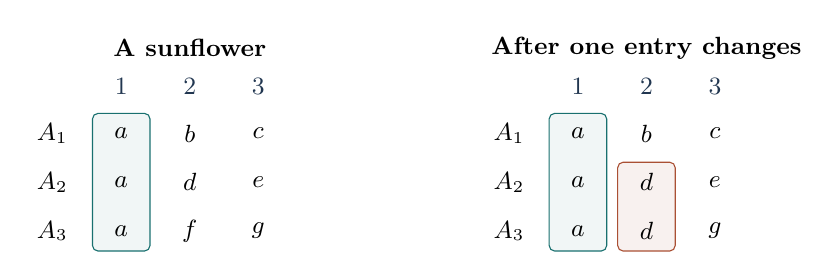
\begin{tikzpicture}[x=.87cm,y=.62cm,font=\small]
  \foreach \offset/\third/\highlight/\heading in {0/f/0/{A sunflower},5.8/d/1/{After one entry changes}}{
    \begin{scope}[xshift=\offset cm]
      \node[font=\small\bfseries] at (2.0,3.75) {\heading};
      \foreach \x in {1,2,3}{\node[text=ink] at (\x,2.96) {\(\x\)};}
      \draw[rounded corners=2pt,draw=sea,fill=sea!6]
                         (.58,-.41) rectangle (1.42,2.41);
      \ifnum\highlight=1
        \draw[rounded corners=2pt,draw=rust,fill=rust!8]
                          (1.58,-.41) rectangle (2.42,1.41);
      \fi
      \foreach \y/\which/\xone/\xtwo/\xthree in
        {2/1/a/b/c,1/2/a/d/e,0/3/a/\third/g}{
        \node[anchor=east] at (.36,\y) {\(A_{\which}\)};
        \node at (1,\y) {\(\xone\)};
        \node at (2,\y) {\(\xtwo\)};
        \node at (3,\y) {\(\xthree\)};
      }
    \end{scope}
  }
\end{tikzpicture}
\caption{In the left family every pair of sets meets in \(\{a\}\).
Changing \(f\) to \(d\) in the last row makes \(A_2\cap A_3=\{a,d\}\).
The other two intersections still equal \(\{a\}\).}\label{fig:columns}
\end{figure}

Call a column \emph{admissible} if it is constant or has all symbols
distinct. In a sunflower-free family, the only ordered \(r\)-tuples
admissible in every column consist of a single repeated word. Indeed,
a column of distinct symbols would make the words distinct, hence give
a sunflower. If every column is constant, the words agree.

The proof turns this observation into a count. Give each of \(r\)
groups of sites an independently chosen word from a family of size \(N\).
At each coordinate apply a tensor operation which kills every partial
repetition and returns a fixed nonzero tensor on a constant column.
These two requirements suffice. Every tuple other than a single repeated word
has a partial repetition somewhere, and the \(N\) repeated-word tuples
all survive. The operations have converted \(r\) independently summed
word labels into a single label shared across the groups.

To measure what this conversion costs, we use a numerical function on
tensors whose value is multiplicative under tensor products and can only
decrease under local linear maps. The logarithm of its value is a
\emph{price}. Sharing a label with \(N\) possible values among the sites
of \(P\) has price \(w(P)\log_2 N\). The Euclidean geometry of the
asymptotic spectrum~\cite{oaG} lets us choose a single price for which
the rates \(w(P)\) are normalized mean widths of the corresponding
sets of points. Place the groups so that the rate for their union
exceeds the sum of their separate rates by \(\rho>0\). The change from
independent labels to a shared one then costs at least \(\rho\log_2 N\).
If the net cost of testing a column is at most \(f\), we obtain
\[
                          \rho\log_2 N\le kf .
\]
The central difficulty is to keep \(f\) bounded for an alphabet of
\emph{any} size. Even two symbols being compared may have arbitrarily
long binary names.

\par\Needspace{7\baselineskip}
\subsection{From a fixed petal count to the quantitative bound}

Part~\ref{part:fixed} proves the fixed-petal bound in the plane. If any
two symbols agree, all remaining symbols must agree with them for the
column to be admissible. Choosing two groups as anchors reduces this
requirement to a list of implications. When the two anchors agree,
they can copy their common symbol directly to a site between them.
The other implications use an equality test that shortens two binary
labels by pairing the alphabet in all possible ways of the form \(\{x,x+p\}\). Two different labels become equal
under exactly one of these pairings. The proof reconstructs and
subtracts that erroneous term. In the planar placement, the net costs
of all the corrections sum to a finite bound even as the label length
grows (Theorem~\ref{thm:filter}). This planar construction already
gives \(\log B_r=O(r^5)\).

Part~\ref{part:quant} obtains the stated dependence on \(r\) by treating
a whole column at once. Its test again shortens each symbol, preserving
every genuine repetition. A partially repeated column can now pass
only by becoming entirely constant. The task is to cancel exactly
those false agreements. The shortened labels are obtained by removing leading bits and
shifting the remaining bits by a mask. If a repeated symbol lies in a
small class with the same leading bits, a recursive test on just that
class pays for the correction. When almost all the active sites outside
the anchors (the satellites) carry the same symbol, splitting those sites into two separated
classes gives a majority in both. The vote in each class can be sent
to a designated site at a cost per output bit governed by one wire
(Lemma~\ref{lem:vote}). The Euclidean placement gives the two votes
together enough width to test their common value against the anchors.
This gives a bound uniform in the alphabet, with \(\log B_r\) bounded
by a polynomial in \(\log r\).
Corollary~\ref{cor:weighted} extends the count to word families that
contain sunflowers. The cost of excluding them is controlled by the rank
of an auxiliary tensor that vanishes on the sunflower tuples and equals
one on the repeated-word tuples.

\subsection{Earlier bounds and related sunflower problems}\label{sec:history}

Erd\H{o}s and Rado suggested replacing the factorial in their 1960
bound by \(c^k\) for an absolute \(c\)~\cite[p.~86]{ER}. In the
notation of Theorem~\ref{thm:main}, this would give \(b_r=O(r)\).
Erd\H{o}s later stated the fixed-petal conjecture explicitly, allowing
the base to depend arbitrarily on \(r\)~\cite[Section~4]{ERstrong}.
For three petals the block-transversal lower bound can be improved.
A construction of Abbott, Hanson and Sauer gives
\(b_3\ge\sqrt{10}\)~\cite{AHS}.

After earlier improvements by Kostochka~\cite{Kostochka}, Alweiss,
Lovett, Wu and Zhang brought the base down to a polylogarithmic
function of \(k\) for fixed \(r\)~\cite{ALWZ}. Their argument finds a
subfamily whose members have a common intersection \(C\), such that
a random subset of the ground set is likely to contain one of the
nonempty remainders \(A\setminus C\). If a random color class in
an \(r\)-coloring contains no remainder with probability less than
\(1/r\), some coloring puts one remainder in each class. These
\(r\) disjoint remainders give the petals. Their examples also show why a logarithmic loss
arises here. For fixed sampling and success probabilities there are
families of size \((\log k)^{(1-o(1))k}\) with no such robust
sunflower~\cite[Section~3]{ALWZ}. Rao's coding argument gave
\(M_r(k)\le (Cr\log(rk))^k\)~\cite{Rao}. Bell, Chueluecha and Warnke
refined the probabilistic step to give \((Cr\log(k+1))^k\)~\cite{BCW}.
Related random-containment estimates enter the study of thresholds of
increasing families~\cite{Thresholds,PP}. Sunflower lemmas also play
a role in Razborov's lower bounds for monotone
circuits~\cite{Razborov}. Rao surveys these connections~\cite{RaoSurvey}.

For \(k\)-uniform families of VC dimension \(d\ge1\), Ge, Wang, Xu and Zhao
obtained the width-independent base \(50dr\)~\cite[Theorem~1.1]{VC},
building on earlier results for restricted set
systems~\cite{FPS,vcsmall}. Shangguan improved the base to
\(O(r\log(d+1))\)~\cite[Corollary~1.4]{Shangguan}. For unrestricted
families Fukuyama proposed a base \(O(r^4)\)~\cite{Fukuyama}.
A product-family obstruction to the sequence-selection estimate in
that argument is described in~\cite{Plasma}.

The size \(N\) of the ground set gives a different measure of the
problem. Erd\H{o}s and Szemer\'edi asked for a bound exponentially
smaller than \(2^N\) on a sunflower-free family of subsets of
an \(N\)-element set~\cite{ES}. Alon, Shpilka and Umans showed how
both conjectures can be studied using words, and that the fixed-petal
conjecture rules out a group construction proposed by Coppersmith
and Winograd for matrix multiplication~\cite{ASU}. Naslund and
Sawin gave a direct slice-rank proof of the ground-set bound for
three petals~\cite{NS}. Buci\'c, He and Lee obtained
\(3(2-1/(16r^3))^N\) for every \(r\ge3\) by polynomial
interpolation~\cite[Theorem~1]{BHL}. For words of length \(k\) over
\(D\) symbols, their bound has base
\((2r)^{2/(r-1)}D^{1-1/(r-1)}\)~\cite[Theorem~2]{BHL}. The
word estimate proved here has a single base for all alphabets, as
required for the passage to \(k\)-element sets on an arbitrary ground
set~\cite[Theorem~2.6]{ASU}.



\par\Needspace{23\baselineskip}
{\small\tableofcontents}

\clearpage
\part{The bound for a fixed number of petals}\label{part:fixed}
\section{From a family of words to a shared label}\label{sec:words}

\subsection{The transversal reduction}
Let \(\W\subseteq\Sigma_1\times\cdots\times\Sigma_k\), where each
alphabet is finite. Arrange an ordered \(r\)-tuple of words as the rows
of an \(r\times k\) array. Call a column \emph{admissible} if its symbols
are all equal or pairwise distinct. If two rows coincide and all columns
are admissible, the repeated entry in each column forces that column to
be constant. Thus an array with admissible columns consists either of a
single repeated word or of \(r\) distinct words. We call \(\W\)
\emph{sunflower-free} if only the first possibility occurs.

A word \(x\) represents the transversal
\(\{(i,x_i):1\le i\le k\}\). Distinct transversals form a sunflower
precisely when every column is admissible. Indeed, a symbol occurring in
two rows of a column belongs to the common intersection and must occur
in every row of that column. Conversely, the constant columns give the
common intersection, and the other columns give disjoint petals.

To find transversals in an arbitrary \(k\)-uniform family \(\F\), color
each ground element independently and uniformly with one of \(k\) colors.
Each member receives all \(k\) colors with probability \(k!/k^k\).
Some coloring therefore retains at least \((k!/k^k)|\F|\) such members.
Reading each retained set in color order identifies it with a word, and
different coordinates use disjoint color classes. Consequently, a bound
\(M^k\) for sunflower-free word families over arbitrary alphabets gives
the set bound \((k^k/k!)M^k\le(eM)^k\). This is the transversal
reduction of Alon, Shpilka and Umans~\cite[Theorem~2.6]{ASU}, based
on the partition argument of Erd\H{o}s and Kleitman~\cite{EK}.

\subsection{The price of sharing a label}
Our starting tensor lets each of \(r\) groups choose a word independently.
Testing the columns will leave one word shared by all groups. To compare
these two tensors we measure the price of sharing one of \(|\W|\)
labels on a prescribed set of sites.

Let \(S\) be a finite set of at least two sites. Tensors belong to
\(\bigotimes_{s\in S}V_s\), with each \(V_s\) a finite-dimensional
vector space over a fixed algebraically closed field of characteristic
\(p>0\). One may take \(p=2\). Positive characteristic enters the degree
constraint in Part~\ref{part:quant}. A \emph{restriction}
\(R\longrightarrow T\) applies one linear map at each site. Tensor
products group the factors at each site. In a direct sum \(R\oplus T\),
the local spaces are direct sums at every site, and the two tensors are
added after inclusion in their respective blocks.

For a nonempty subset \(P\subseteq S\), put
\[
       E_P(j)=\bigotimes_{s\in P}e_j,\qquad
       G_P(L)=\sum_{j=1}^{L}E_P(j),
\]
with scalar factors \(1\) outside \(P\). In each summand of \(G_P(L)\),
every site in \(P\) holds the same basis label \(j\). We call this tensor
a \emph{diagonal}, or a partial diagonal when \(P\ne S\). Its basis
labels can equally well be the members of a word family of size \(L\).

A \emph{spectral point} \(\varphi\) assigns nonnegative real values to
tensors. It takes zero to zero and the scalar unit to one, is monotone
under restriction, multiplies on tensor products and adds on direct
sums~\cite{Strassen}. Every nonzero tensor restricts to the unit.
Its \emph{price} \(h(T)=\log_2\varphi(T)\) is therefore nonnegative.
Define \(w(P)=h(G_P(2))\), the price of one bit shared on \(P\). Then
\begin{equation}\label{eq:price}
       h(G_P(L))=w(P)\log_2 L,\qquad 0\le w(P)\le w(S)=1 .
\end{equation}
Indeed, tensoring diagonals multiplies their label counts, and a local
projection can discard any set of labels. Compare \(L^m\) with the
two neighboring powers of two, take prices, divide by \(m\), and let
\(m\) tend to infinity. Sending each \(e_j\) to \(1\) at a site removes
that site from the shared label, so \(w(P)\) is monotone in \(P\).
The full diagonal \(G_S(2)\) is the direct sum of two units. At a
single site the diagonal is a nonzero vector and its price is zero.

\subsection{The comparison}
A site that holds a basis label \(x\) can use it as a \emph{control}.
For any family of linear maps \(M_x\) with common domain and codomain,
the assignment
\[
             e_x\otimes v\longmapsto e_x\otimes M_xv
\]
defines a single linear map. Thus the site can read a coordinate of
its word, keep the word label, and use the symbol to choose the next
operation. The same prescription acts term by term on a sum. Operations
can write fresh basis labels as controls for later maps. Adding two
restrictions with common output spaces uses the direct sum of their
inputs. To subtract the second output, multiply its block by \(-1\)
at one site.

Partition \(S\) into \(r\) nonempty groups, and assign one symbol to
each group. For three distinct groups, the rule \((U,V)\to W\) says
that when \(U\) and \(V\) agree, \(W\) must have their common symbol.
A list of rules \emph{forces admissibility} if every assignment
satisfying them gives an admissible column. A test for a rule starts
with an auxiliary tensor \(R\). At selected sites of the three groups,
the group symbol controls a local map. If all three symbols agree, the
test must return a prescribed nonzero tensor \(Q\). Its \emph{net cost}
is \(h(R)-h(Q)\). The spaces, \(R\), and \(Q\) are fixed independently
of the values of the controls.

\begin{proposition}[Comparison of independent and shared labels]\label{prop:comparison}
Fix a spectral point and a partition of \(S\) into \(r\) groups with
\(\rho=w(S)-\sum_J w(J)>0\). Suppose a list of rules forces admissibility.
For each rule \(j\) and every finite alphabet, suppose there is a test
of net cost at most \(c_j\) that returns its fixed tensor whenever the
three symbols agree and returns zero whenever the rule is violated.
Then every nonempty sunflower-free word family of length \(k\) satisfies
\[
                 \rho\log_2|\W|\le k\sum_j c_j .
\]
\end{proposition}

\begin{proof}
Write \(N=|\W|\). The tensor \(\bigotimes_J G_J(N)\) has one summand
for every independent choice of a word in \(\W\) at each group \(J\).
Supply a separate test for each rule in each column, and let \(R\) and
\(Q\) denote the products of their input and return tensors. On each
summand, run the tests controlled by the symbols of the chosen words,
retaining the word labels.

An \(r\)-tuple other than a repeated word has an inadmissible column,
because \(\W\) is sunflower-free. Some rule there is violated. Its
zero output kills the entire summand, whatever the other tests return.
On a repeated word every test returns its prescribed tensor. Summing
over the surviving words gives the restriction
\[
        \left(\bigotimes_J G_J(N)\right)\otimes R
                 \longrightarrow G_S(N)\otimes Q .
\]
By monotonicity and Equation~\eqref{eq:price}, sharing the word across
all groups increases its price by \(\rho\log_2 N\). This increase
is at most \(h(R)-h(Q)\le k\sum_j c_j\).
\end{proof}

\subsection{Choosing the prices by a Euclidean placement}
Proposition~\ref{prop:comparison} asks for weights with a positive
surplus \(\rho\) and with bounded costs for the tests. We choose them
by placing the sites in Euclidean space. For a finite nonempty set
\(P\subset\R^d\) or its convex hull, put
\[
    \delta(P)=\sqrt{2\pi}\,\E\max_{x\in P}\langle G,x\rangle,
    \qquad G\sim N(0,I_d).
\]
This normalization of Gaussian mean width gives zero on a point and
Euclidean length on a segment, since \(\sqrt{2\pi}\,\E(G_1)_+=1\).
It is translation invariant and additive under Minkowski sums.
In the plane it is the semiperimeter of the convex hull, with a
degenerate segment counted twice in the perimeter.

\begin{theorem}[Euclidean prices {\cite[Theorem~\ext{G}{thm:main} and Section~\ext{G}{sec:spectra}]{oaG}}]\label{thm:flat}
For any field and any finite set of distinct sites \(S\subset\R^d\)
with \(D=\delta(S)>0\), there is a spectral point on tensors on \(S\)
over that field for which
\[
                   w(P)=\frac{\delta(P)}{D}
                   \qquad(\varnothing\ne P\subseteq S).
\]
\end{theorem}

We take the point induced by the compatible Euclidean assignment
of~\cite{oaG}. Thus a single evaluation prices every shared label in
the comparison. Section~\ref{sec:plane} uses semiperimeters to choose
the groups and the sites read by each rule. Section~\ref{sec:degree}
uses the joint convexity, isometry invariance and dilation law of the
same assignment to price a total-degree constraint.

\section{A planar proof for a fixed number of petals}\label{sec:plane}
Proposition~\ref{prop:comparison} asks for a placement with two properties.
Sharing a word among all \(r\) groups must cost more than sharing it
within the groups separately. At the same time, checking the agreement
rules must have bounded cost in each coordinate, however large its
alphabet. We will place two groups on line segments and the other
\(r-2\) groups at points between them. In this placement, comparing
two symbols already shared over suitable groups of sites costs a bounded
amount.

\subsection{Comparing and copying shared symbols}
Fix a spectral point \(\varphi\) on \(S\). Let \(P,T\subseteq S\) be
disjoint nonempty sets of sites and put \(K=P\cup T\). Each site of \(K\)
receives a \(b\)-bit control. An \emph{equality filter} consists of
fixed nonzero input and return tensors \(R,Q\) and controlled local maps.
When the sites of \(P\) all read \(x\) and those of \(T\) all read \(y\),
the maps must take \(R\) to \(\mathbf 1_{\{x=y\}}Q\). On any other
assignment of the controls the output is unrestricted. Denote by
\(c_b(P,T)\) the infimum of the net costs \(h(R)-h(Q)\).
Taking \(b=\lceil\log_2|\Sigma|\rceil\) accommodates any finite alphabet
\(\Sigma\). A one-symbol alphabet needs no test.

\par\Needspace{6\baselineskip}
\begin{theorem}[Equality testing]\label{thm:filter}
Put \(g=w(P)+w(T)-w(K)\), \(g_-=\max\{0,-g\}\), and
\(\ell=\log_2(2|K|)\). For every \(b\ge1\),
\[
        g_- b\ \le\ c_b(P,T)\
             \le\ g_- b+Cw(K)\sqrt{b\ell}.
\]
In particular the cost per bit tends to \(g_-\). When \(g>0\), there
is an equality filter of net cost at most \(Cw(K)^2\ell/g\) for every
\(b\), where \(C\) is an absolute constant.
\end{theorem}

For an implication \((U,V)\to W\), let \(P\) read sites in both \(U,V\)
and let \(T\) read sites in \(W\). When the implication fails, \(P\)
reads one symbol and \(T\) a different one, so the filter gives zero.
When all three symbols agree it returns \(Q\). Thus a positive \(g\)
gives exactly the alphabet-independent guarantee of
Proposition~\ref{prop:comparison}. Sections~\ref{sec:copy} and~\ref{sec:filter}
prove the equality estimate. We will also need a second way to enforce
an implication when the target lies between the two sources.

\begin{lemma}[Copying inside a convex hull]\label{lem:segment}
Let \(P,Z\) be disjoint nonempty sets of sites with \(w(P\cup Z)=w(P)\).
For every \(N\ge1\), a controlled restriction on \(P\) returns
\(Q\otimes E_Z(i)\) whenever all sites of \(P\) read \(i\in[N]\),
for a fixed nonzero tensor \(Q\). Its net cost is at most
\(w(P)\log_2(|Z|+2)\). For the Euclidean spectral point of
Theorem~\ref{thm:flat}, the width condition holds whenever
\(Z\subseteq\conv(P)\).
\end{lemma}
\begin{proof}
Write \(c=|Z|\). Choose \(L\) from \(c+1,c+2\) so the characteristic
does not divide \(L\), and let \(\zeta\) be a primitive \(L\)-th root
of unity. Supply \(G_{P\cup Z}(L^N)\), indexing the shared basis by
\(t=(t_1,\ldots,t_N)\in(\mathbb Z/L\mathbb Z)^N\). When a source
reads \(i\), it deletes \(t_i\) and keeps the other coordinates in
order. One source also multiplies by \(L^{-1}\zeta^{-ct_i}\).
Each target maps \(e_t\) to \(\sum_{j=1}^N\zeta^{t_j}e_j\).

Fix the retained source index and a tuple of target indices
\((j_z)_{z\in Z}\). If \(m\) of them equal \(i\), summation over \(t_i\)
contributes the factor \(L^{-1}\sum_{s=0}^{L-1}\zeta^{(m-c)s}\).
This is zero unless \(m=c\), since \(0\le m\le c<L\).
When \(m=c\) all phases cancel, leaving coefficient one. The output is
therefore \(G_P(L^{N-1})\otimes E_Z(i)\). With \(w(P\cup Z)=w(P)\),
Equation~\eqref{eq:price} gives net cost \(w(P)\log_2 L\).
\end{proof}

\subsection{The placement and its agreement rules}
Name the two anchor groups \(A,B\) and the remaining groups
\(Z_1,\ldots,Z_{r-2}\). In each coordinate use the rules
\begin{equation}\label{eq:rules}
 (A,B)\to Z_i,\qquad (A,Z_i)\to B,\qquad (B,Z_i)\to A,
 \qquad (Z_i,Z_j)\to A\quad(i<j).
\end{equation}
If the anchors agree, the first rules force agreement everywhere. An
agreeing anchor and satellite force the other anchor to agree. Two
agreeing satellites first force agreement with \(A\), which in turn
forces agreement with \(B\). Thus a column satisfying the rules is
either constant or pairwise distinct.

Set
\[
   t=\frac{1}{2(r-1)},\qquad \eta=\frac{t^2}{4},\qquad
   y_i=1-\frac{i}{r-1}\quad (1\le i\le r-2).
\]
The anchors occupy the ends of two vertical unit segments at horizontal
coordinates \(0\) and \(1+\eta\), together with the sites
\(a_i=(0,y_i)\) and \(b_i=(1+\eta,y_i)\) on those segments.
Group \(Z_i\) occupies the single site \((t,y_i)\). The whole placement
has semiperimeter \(D=2+\eta\). By Theorem~\ref{thm:flat}, a group
\(P\) has weight \(w(P)=\delta(P)/D\), with \(\delta(P)\) its
semiperimeter. Only the anchors contribute to the sum of group weights,
so the surplus for Proposition~\ref{prop:comparison} is
\[
              \rho=1-\frac{2}{2+\eta}=\frac{\eta}{2+\eta}>0 .
\]

\begin{figure}[htb]
\centering
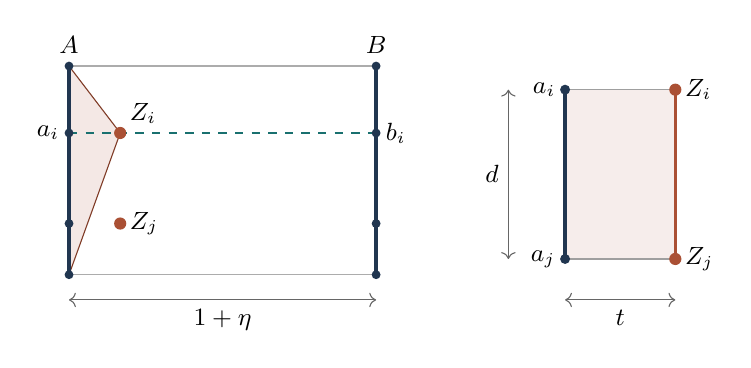
\begin{tikzpicture}[x=1cm,y=1cm,font=\small]
  \begin{scope}
    \draw[gray!65] (0,0) rectangle (3.9,2.65);
    \fill[rust!13] (0,0)--(.65,1.8)--(0,2.65)--cycle;
    \draw[rust!75!black] (0,0)--(.65,1.8)--(0,2.65);
    \draw[very thick,ink] (0,0)--(0,2.65) (3.9,0)--(3.9,2.65);
    \draw[sea,thick,dashed] (0,1.8)--(3.9,1.8);
    \foreach \x in {0,3.9}{\foreach \y in {0,.65,1.8,2.65}
      {\fill[ink] (\x,\y) circle(1.6pt);}}
    \node[above] at (0,2.68) {\(A\)};
    \node[above] at (3.9,2.68) {\(B\)};
    \node[left] at (0,1.8) {\(a_i\)};
    \node[right] at (3.9,1.8) {\(b_i\)};
    \fill[rust] (.65,1.8) circle(2.2pt) node[above right,text=black] {\(Z_i\)};
    \fill[rust] (.65,.65) circle(2.2pt) node[right,text=black] {\(Z_j\)};
    \draw[<->,gray!80!black] (0,-.32)--node[below,text=black]{\(1+\eta\)}(3.9,-.32);
  \end{scope}
  \begin{scope}[xshift=6.3cm]
    \fill[rust!10] (0,.2) rectangle (1.4,2.35);
    \draw[gray!75] (0,.2) rectangle (1.4,2.35);
    \draw[very thick,ink] (0,.2)--(0,2.35);
    \draw[very thick,rust] (1.4,.2)--(1.4,2.35);
    \foreach \y/\lab in {2.35/i,.2/j}{
      \fill[ink] (0,\y) circle(1.8pt) node[left,text=black]{\(a_{\lab}\)};
      \fill[rust] (1.4,\y) circle(2.2pt) node[right,text=black]{\(Z_{\lab}\)};}
    \draw[<->,gray!80!black] (-.72,.2)--node[left,text=black]{\(d\)}(-.72,2.35);
    \draw[<->,gray!80!black] (0,-.32)--node[below,text=black]{\(t\)}(1.4,-.32);
  \end{scope}
\end{tikzpicture}
\caption{At left, \(a_i\) and \(b_i\) can copy a common symbol to
\(Z_i\) on their joining segment. The shaded triangle is the convex hull of \(A\cup\{Z_i\}\),
whose semiperimeter exceeds that of \(A\).
At right, the four sites used to check \((Z_i,Z_j)\to A\)
form a rectangle with \(d=|y_i-y_j|>t\).}
\label{fig:placement}
\end{figure}

For \((A,B)\to Z_i\), read \(a_i\) and \(b_i\). Their segment contains
\(Z_i\), as in Figure~\ref{fig:placement}. Lemma~\ref{lem:segment}
copies their common label to \(Z_i\) at bounded cost. The local map
there accepts the copied label precisely when it equals the satellite's
own control.

For \((Z_i,Z_j)\to A\), use \(P=\{Z_i,Z_j\}\) and \(T=\{a_i,a_j\}\).
Both segments have length \(d=|y_i-y_j|\ge2t\), and their union spans
the rectangle in Figure~\ref{fig:placement}. The corresponding
semiperimeter gap is \(2d-(d+t)=d-t\ge t\). Theorem~\ref{thm:filter}
applies with \(g=(d-t)/D\). For \(r=3\) there is only one satellite
and no rule of this type.

For \((A,Z_i)\to B\), let \(P\) contain \(Z_i\) and the endpoints of
\(A\), and let \(T\) consist of the endpoints of \(B\). Adding a point
at height \(y\in[0,1]\) and horizontal distance \(s\) from a unit
segment increases its semiperimeter by
\[
  \frac{\sqrt{y^2+s^2}+\sqrt{(1-y)^2+s^2}-1}{2}
     \ \ge\ \frac{\sqrt{1+4s^2}-1}{2} .
\]
The inequality follows from the triangle inequality applied to
\((y,s)\) and \((1-y,s)\). Here \(s=t\). For \((B,Z_i)\to A\) the
same calculation uses \(s=1+\eta-t\ge t\). In either case the
increase is at least
\(2t^2/(\sqrt{1+4t^2}+1)>t^2/2\), since \(t\le1/4\).
The two anchors together span the whole rectangle. Subtracting its
semiperimeter \(2+\eta\) leaves a gap greater than \(t^2/2-\eta=\eta\).
Thus both filters have \(g>\eta/D\).

Each filter just used reads at most five sites. The \(O(r)\) rules
with a satellite and an anchor as antecedents therefore cost \(O(r^2)\)
each, and the \(O(r^2)\) satellite-pair rules cost \(O(r)\) each.
Copying from the two anchors costs \(O(1)\) per satellite.
Since \(\rho\) is of order \(r^{-2}\), Proposition~\ref{prop:comparison}
gives \(\log_2|\W|=O(r^5 k)\). The transfer in Section~\ref{sec:words}
adds only \(O(k)\) to this logarithm for set families.
This already gives an exponential bound in \(k\) for every fixed \(r\).
Part~\ref{part:quant} obtains the stronger dependence on \(r\) by
testing many implications together.

\section{Broadcasting a shared label}\label{sec:copy}

Suppose that every source in \(P\) knows the same \(b\)-bit label \(x\).
To send \(x\) to a set \(Z\) of new sites, one source can select the
\(x\)-term of a diagonal shared by \(P\cup Z\). This costs \(w(P\cup Z)b\).
Agreement across the sources lets us recover a diagonal on \(P\) in the
same operation. The returned diagonal has price \(w(P)b\).
This use of a readable label is related to
\cite[Proposition~\ext{G}{lem:submod}]{oaG}.

\begin{lemma}[Broadcasting]\label{lem:copy}
Fix a spectral point on \(S\), disjoint nonempty sets \(P,Z\subseteq S\),
and an integer \(b\ge1\). Put \(K=P\cup Z\), \(N=2^b\), and
\(\ell=\log_2(2|K|)\). Give each site of \(P\) a control in \([N]\).
There are an input tensor \(R\) and controlled local maps that return
\(G_P(N)\otimes E_Z(x)\) whenever the controls all equal \(x\), with
\[
 h(R)-h(G_P(N))
       \le (w(K)-w(P))b+O\!\left(w(K)\sqrt{b\ell}\right).
\]
The implied constant is absolute. Any such conversion returning
\(Q\otimes E_Z(x)\) with \(Q\) fixed and nonzero has net cost at least
\((w(K)-w(P))b\).
\end{lemma}

\begin{proof}
For the lower bound, supply the common control as the coherent sum
\(G_P(N)\) and retain its local basis vectors. Term by term, the conversion
extends the common label to \(Z\). Thus
\(G_P(N)\otimes R\longrightarrow G_K(N)\otimes Q\), and monotonicity
gives the bound.

For the construction, write \(a=|P|\) and \(c=|Z|\). The elementary
broadcast described above selects \(x\) at one source and sends every
basis vector to \(1\) at the others. Carry an independent \(G_P(N)\)
through this operation. Its net cost \(w(K)b\) suffices when \(a=1\),
since then \(w(P)=0\). It also suffices when \(b\le\ell\), since then
\(w(P)b\le w(K)\sqrt{b\ell}\). Henceforth \(a\ge2\) and \(b>\ell\).

We encode the broadcast label and the returned diagonal by integer
vectors. In a box \(V=\{0,\ldots,q-1\}^m\), choose a set \(H\) of
\(N\) vectors with the same Euclidean norm and identify \([N]\) with \(H\).
For each \(u\in H\), choose an ordered set \(V_u\subseteq V\) of \(N\)
vectors having the same norm and the same inner product with \(u\).
We choose \(q,m\) below. On control \(u\), source \(j\) will output
the index of a vector \(v_j\in V_u\), and target \(z\) will output
the label \(g_z\in H\). Impose the single vector equation
\begin{equation}\label{eq:broadcast-relation}
  \sum_{z\in Z}g_z=cu+\sum_{j=2}^a v_j-(a-1)v_1 .
\end{equation}

Taking the inner product with \(u\) cancels all the terms involving
\(v_j\). It gives \(\sum_z\langle u,g_z\rangle=c\|u\|^2\).
Since every \(g_z\) has the norm of \(u\), equality forces \(g_z=u\)
for every \(z\). Equation~\eqref{eq:broadcast-relation} now says that
\(v_1\) is the average of the other source vectors. Their equal norms
give \(\sum_{j=2}^a\|v_j-v_1\|^2=0\). Conversely, every
\(v\in V_u\) gives a solution with all \(v_j=v\) and all \(g_z=u\).
Summing over the solutions therefore returns exactly \(N\) diagonal
terms on \(P\), each with the desired label at every site of \(Z\).
The use of a sphere to force equality in an average is the geometric
step in Behrend's construction~\cite{Behrend}.

To impose the equation by local maps, take \(L=(a+c-1)(q-1)+1\),
increasing it by one if the characteristic divides it. Write
\(\Gamma=(\mathbb Z/L\mathbb Z)^m\). In every coordinate the two
sides of Equation~\eqref{eq:broadcast-relation} differ by less than
\(L\) in absolute value. Their equality can therefore be tested in
\(\Gamma\). For \(D\in\Gamma\) the indicator of \(D=0\) is
\(|\Gamma|^{-1}\sum_{\chi\in\widehat\Gamma}\chi(D)\), since the
field contains all \(L\)-th roots of unity and \(L\) is invertible.

Supply \(R=G_K(|\Gamma|)\) with its shared index named by \(\chi\).
Each target sums over its possible \(g_z\) with coefficient \(\chi(g_z)\).
Each source \(j\ge2\) sums over \(v_j\in V_u\) with coefficient
\(\chi(-v_j)\), and source \(1\) uses
\(|\Gamma|^{-1}\chi((a-1)v_1-cu)\).
The product of these coefficients is the character summand for the
difference of the two sides. Each output index is the basis label
specified above, so character orthogonality gives
\(G_P(N)\otimes E_Z(u)\). Only the source maps use a control.

It remains to choose a small enough group. Set
\[
 d=\lceil\sqrt{b\ell}\rceil+4,\qquad q=2^d,\qquad
 m=\lceil b/d\rceil+6 .
\]
The squared norm of a point in \(V\) and its inner product with a
fixed \(u\in V\) each take at most \(B=1+m(q-1)^2\le q^3\) values,
since \(m\le d+6\le q\). Pigeonholing by norm gives \(H\), and
pigeonholing by both statistics gives every \(V_u\), because
\(|V|/B^2\ge q^{m-6}\ge 2^b\). Finally \(\log_2 L\le d+\ell\) and
\[
 \log_2|\Gamma|\le (b/d+7)(d+\ell)
                  \le b+O(\sqrt{b\ell}).
\]
Subtracting the price \(w(P)b\) of the returned diagonal gives the
claimed net cost.
\end{proof}

\section{Constructing the equality test}\label{sec:filter}

On the promise of Theorem~\ref{thm:filter}, let \(x\) be the label
shared by \(P\) and \(y\) the label shared by \(T\). A perfect matching
on the alphabet contracts each pair to a single name, cutting the
number of bits by one. We will run the shorter equality test on a
family of such matchings. When \(x\ne y\), exactly one matching
pairs them. Its index can be computed by two broadcasts, so the
resulting false match can be cancelled exactly.

\begin{proof}[Proof of Theorem~\ref{thm:filter}]
Put \(K=P\cup T\) and \(g=w(P)+w(T)-w(K)\).
Fixed equal controls take \(R\) to \(Q\), so every filter has
nonnegative cost. Supply the two controls independently as
\(G_P(2^b)\otimes G_T(2^b)\), retaining their local indices.
The filter kills all terms with different labels, giving
\[
 G_P(2^b)\otimes G_T(2^b)\otimes R
       \longrightarrow G_K(2^b)\otimes Q .
\]
Taking prices gives the second lower bound \(h(R)-h(Q)\ge -gb\).

We construct the upper bound first for \(S=K\), so \(w(K)=1\).
Fix a bit length \(b\ge1\). The labels form the set \(\mathbb F_2^b\),
regardless of the characteristic of the tensor field. For each
nonzero \(p\), the pairs \(\{x,x+p\}\) form a perfect matching.
Name its pairs by \((b-1)\)-bit strings and write \(\pi_p(x)\)
for the name of the pair containing \(x\). If \(x=y\), the names
agree in every matching. If \(x\ne y\), they agree precisely when
\(p=x+y\). Keeping the index of each surviving matching gives the
identity
\[
 \sum_{\substack{p\ne0\\ \pi_p(x)=\pi_p(y)}} E_K(p)
 =
 \begin{cases}
 G_K(2^b-1), & x=y,\\
 E_K(x+y),   & x\ne y .
 \end{cases}
\]

We need a correction producing the second line on unequal inputs and
zero on equal inputs. Broadcast \(x\) from \(P\) to \(T\) by
Lemma~\ref{lem:copy}. At each site of \(T\) the control \(y\)
selects the map \(e_x\mapsto e_{x+y}\) for \(x\ne y\) and
\(e_y\mapsto0\). Keep this new basis label at \(T\) and use it as
the common control for a second broadcast from \(T\) to \(P\).
Denote the tensor products of the two input resources and the two
returns by \(U_b\) and \(V_b\), respectively. On unequal inputs
the output is \(V_b\otimes E_K(x+y)\). All its label slots may be
projected onto the span of the nonzero indices. With
\(\ell=\log_2(2|K|)\), Lemma~\ref{lem:copy} gives
\begin{equation}\label{eq:filter-correction}
 h(U_b)-h(V_b)\le (1-g)b+C_0\sqrt{b\ell}.
\end{equation}
Indeed, the two leading costs add to
\((1-w(P))b+(1-w(T))b=(1-g)b\).

Start the recursion with \(R_0=Q_0=1\). At bit length \(b\), let
\(L_b=2^b-1\) and give every site access to the same matching index
through \(G_K(L_b)\). The shorter filter on the two pair names
can be applied under control of this index. With \(p\) retained,
its output on equal labels contains the entire \(G_K(L_b)\).
Including that diagonal in the return leads to the following choice
of resources for the two branches.
\begin{align*}
 Q_b &= Q_{b-1}\otimes V_b\otimes G_K(L_b),\\
 R_b &= \bigl(R_{b-1}\otimes V_b\otimes G_K(L_b)\bigr)
             \oplus \bigl(Q_{b-1}\otimes U_b\bigr).
\end{align*}
The first summand runs the shorter filter, keeps \(V_b\), and
returns \(Q_b\) on equal controls. On unequal controls its output is
\(Q_{b-1}\otimes V_b\otimes E_K(x+y)\). The second summand retains
\(Q_{b-1}\) and forms exactly this correction, with zero output on
equal controls. Multiply its map at one site by \(-1\).
Both sets of local maps now land in the same spaces, so their maps on
the local direct sums produce the difference. This eliminates the
single false match in every characteristic.

Set \(f_b=\varphi(R_b)/\varphi(Q_b)\). The diagonal of \(L_b\)
matchings is furnished and returned by the recursive branch. Thus
only the correction contributes a new term to the price ratio.
Additivity on direct sums and Equation~\eqref{eq:filter-correction}
give
\[
 f_0=1,\qquad
 f_b=f_{b-1}+\frac{\varphi(U_b)}{L_b\varphi(V_b)}
      \le f_{b-1}+2^{1-gb+C_0\sqrt{b\ell}} .
\]
Here \(L_b\ge 2^{b-1}\). Each of the first \(b\) increments is at most
\(2^{1+\max\{0,-g\}b+C_0\sqrt{b\ell}}\). Taking logarithms of their
sum with \(f_0\) and using \(\log_2(b+1)=O(\sqrt b)\) yields
\[
 \log_2 f_b\le\max\{0,-g\}b+C_1\sqrt{b\ell}
\]
with absolute \(C_1\). When \(g>0\), the entire series is bounded.
Indeed, \(C_0\sqrt{b\ell}\le gb/2+C_0^2\ell/(2g)\) gives
\[
 f_b\le 1+\frac{2^{1+C_0^2\ell/(2g)}}{2^{g/2}-1}.
\]
Since \(0<g\le1\) and \(\ell\ge1\), this gives
\(\log_2 f_b=O(\ell/g)\) with an absolute constant.

To place this filter in the original set of sites \(S\), put
\(\theta=w(K)\). If \(\theta=0\), the tensor \(G_K(2^b)\) has price
zero. One site in each group selects its control index from that
diagonal and the other sites send every index to \(1\), giving
\(\mathbf 1_{\{x=y\}}\) at zero cost.

Suppose \(\theta>0\). Write \(\iota X\) for a \(K\)-tensor padded by
scalar factors on \(S\setminus K\). Then
\(\psi(X)=\varphi(\iota X)^{1/\theta}\) is a spectral point on \(K\)
\cite[Section~\ext{G}{sec:spectra}]{oaG}. To see additivity, expand
\((X\oplus_K Y)^{\otimes m}\) and group terms by their number \(j\) of
\(X\)-factors. The \(j\)-th group is locally isomorphic to
\[
 G_K\!\left(\binom mj\right)
       \otimes X^{\otimes j}\otimes Y^{\otimes(m-j)}.
\]
Each group can be extracted by a projection. The direct sum on \(S\)
of all the padded groups restricts to the padded power by identifying
the scalar slots outside \(K\). Hence \(\varphi(\iota(X\oplus_K Y))^m\)
lies between the largest group value and \(m+1\) times that value.
By Equation~\eqref{eq:price}, the \(1/\theta\) power of the \(j\)-th value
is \(\binom mj\psi(X)^j\psi(Y)^{m-j}\). Its maximum differs from
the binomial sum by at most a factor \(m+1\). Taking \(m\)-th roots
proves additivity. The remaining spectral axioms follow from those
of \(\varphi\).

Under \(\psi\) the gap on \(K\) is \(g/\theta\). Padding the filter
constructed there multiplies its net cost by \(\theta\). Thus for
every \(b\ge1\) its cost on \(S\) exceeds \(\max\{0,-g\}b\) by at
most \(C_1 w(K)\sqrt{b\ell}\), and for \(g>0\) it is bounded by
\(O(w(K)^2\ell/g)\) uniformly in \(b\). The lower bounds proved
above then give the limiting cost per bit.
\end{proof}


\par\Needspace{15\baselineskip}
\part{The dependence on the number of petals}\label{part:quant}
\section{Testing a column with many symbols}\label{sec:design}

In the planar proof an implication is tested for every possible pair
of equal symbols. A column with \(r\) entries has \(\binom r2\) such
pairs. To obtain the bound of Theorem~\ref{thm:main} with its stated
dependence on \(r\), we construct a single test for the whole column.
It returns a fixed nonzero tensor on agreement and vanishes on every
\emph{violation}, meaning that some symbol repeats but the column is
nonconstant. Its value on pairwise distinct symbols may be arbitrary.

Take \(r\ge4\). Write \(H=\log(2r)\) and \(L=\log(2H)\), with all
logarithms in base two. Two of the symbols are held on groups of sites
\(A,B\), called the anchors. The other symbols are held at individual
satellite sites. The recursive test will sometimes use only a subset
of the satellites, called the active satellites. The two anchors have
joint width one and individual widths summing to \(1-s\). Since the
satellites are points, this leaves a surplus \(s>0\) in the word-count
comparison of Section~\ref{sec:words}. We seek a bound on the cost of
one column that is independent of the length of its symbols.

\paragraph{Shortening a symbol.}
Split each symbol into a head \(a\) and a tail \(v\) of \(b'\) bits.
For every possible head, sum over a mask \(m_a\) of \(b'\) bits shared
by all sites. Apply the shorter test to the column of shifted tails
\(v+m_a\), with bitwise addition modulo two. Retain the masks in the
output. On agreement every choice of masks survives, so the test
returns their full diagonals. On a violation the repeated symbol stays
repeated. The shorter test can therefore survive only if all the
shifted tails take a single value \(z\). We have to subtract the masks
producing this \emph{false tie}.

For a given \(z\), every entry \((a,v)\) forces \(m_a=v+z\). If two
tails at one head disagree, there is no solution. An empty head
leaves its mask free. Figure~\ref{fig:example} gives a five-entry
column in which only the two satellites \(P,R\) repeat a letter.
At \(z=01\), the two occurrences of head \(10\) both require
\(m_{10}=10\).

\begin{figure}[!htbp]
\centering
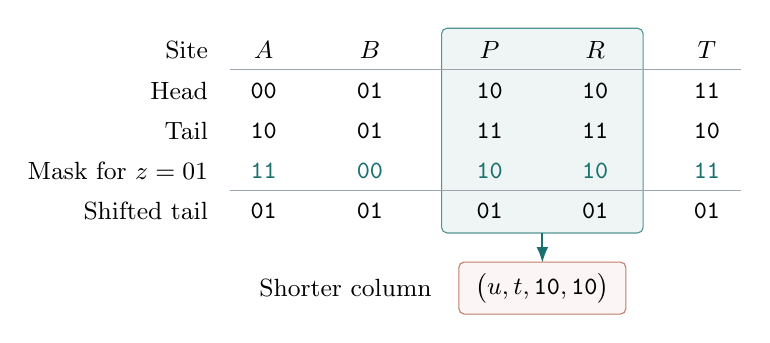
\begin{tikzpicture}[x=1cm,y=1cm,font=\small,
 lab/.style={anchor=east,inner sep=0pt},bit/.style={font=\small\ttfamily},
 line/.style={draw=ink!45},child/.style={draw=rust!75,fill=rust!5,
 rounded corners=2pt,inner xsep=6pt,inner ysep=4pt}]
 \fill[sea!7,rounded corners=2pt] (2.26,-.32) rectangle (4.82,2.28);
 \draw[sea!75,rounded corners=2pt] (2.26,-.32) rectangle (4.82,2.28);
 \foreach \y/\name in {2/Site,1.49/Head,.98/Tail,.47/Mask for \(z=01\),-.04/Shifted tail}
   \node[lab] at (-.7,\y){\name};
 \foreach \x/\site/\head/\tail/\mask in
   {0/A/00/10/11,1.35/B/01/01/00,2.87/P/10/11/10,4.21/R/10/11/10,5.63/T/11/10/11}{
    \node at (\x,2){\(\site\)};
    \node[bit] at (\x,1.49){\head};
    \node[bit] at (\x,.98){\tail};
    \node[bit,text=sea] at (\x,.47){\mask};
    \node[bit] at (\x,-.04){01};
 }
 \draw[line] (-.43,1.76)--(6.06,1.76);
 \draw[line] (-.43,.22)--(6.06,.22);
 \draw[-{Latex[length=2mm]},thick,sea] (3.54,-.32)--(3.54,-.7);
 \node[child] at (3.54,-1.02) {\(\bigl(u,t,\mathtt{10},\mathtt{10}\bigr)\)};
 \node[lab] at (2.14,-1.02){Shorter column};
\end{tikzpicture}
\caption{One false tie and its correction. The shaded satellites carry
the same original symbol. Their required mask becomes their input in
the shorter column, alongside the two auxiliary anchor inputs \(u,t\).
The repeat forces this column to pass only at \(u=t=\mathtt{10}\).
The sum over \(u,t\) thus recovers the required mask.}
\label{fig:example}
\end{figure}

\paragraph{Recovering the cost of a false tie.}
We could supply every mask, sum over \(z\), and check the constraints
\(m_a=v+z\) locally. Relative to the mask diagonals returned on
agreement, this would leave \(b'\) bits to pay for \(z\). First
consider a violation in which neither anchor symbol repeats. At a
false tie each anchor must be alone in its head, since every entry in
a given head must have the same tail. Each anchor can therefore
compute its mask locally from \(z\) and broadcast it. A broadcast
from \(A\) to all sites costs \((1-w(A))b'\), saving \(w(A)b'\) against
the full mask diagonal. The two anchors together pay for
\((1-s)b'\) of the cost of \(z\). This leaves \(sb'\).

A head containing a genuine satellite repeat can cover the remainder.
Give two auxiliary anchor groups independent dummy labels \(u,t\);
their widths sum to \(1-s'\), with \(s'\ge s\). For each active
satellite in the chosen head, give the shorter test its required mask
\(v+z\). If a whole symbol repeats in that head, the shorter column
has a repeat for every pair \(u,t\). If its required masks differ, it
always vanishes. If the masks agree, exactly one pair \(u,t\) makes
the shorter column constant. The auxiliary anchors can then broadcast
their common label from their joint width of one. The cost of the two
dummy labels saves \(s'b'\) against the full mask diagonal, before
the cost of the shorter test itself.

Inclusion--exclusion removes the need to identify the repeated head. Let
\(I_i\) be the exact mask operation for head \(i\), and let \(T_i\) be
the operation using the shorter test, with the auxiliary tensor
factors made common to the terms. With two possible non-anchor heads,
use
\[
          I_0\otimes I_1-(I_0-T_0)\otimes(I_1-T_1).
\]
At a repeated symbol in head \(i\) we have \(T_i=I_i\), so the
display equals the exact mask correction. When the product is
expanded, every remaining term uses at least one shorter test.
Section~\ref{sec:masks} carries out this cancellation for any number
of heads, keeping each mask tuple in its own output slot.

\paragraph{Controlling the size of the shorter test.}
A preliminary gate, the \emph{guard}, handles violations with a
repeated anchor symbol. It also kills a violation when one symbol
occurs at more than \((1-p_0)n\) of the \(n\) active satellites, for
a fixed \(p_0>0\). On a surviving violation a head larger than this
threshold cannot have a common tail. Its exact correction is then
zero, and we can omit the shorter test at that head. Thus a recursive
call that changes the active satellites always reduces their number
by a fixed fraction.

The difficulty in implementing the guard is to compare a widely
repeated symbol with the anchors without sending every satellite
symbol to them. On the guard's large-majority promise, a balanced split of the active
satellites into two geometrically separated classes leaves the same
symbol in a strict majority in each class. For any projection of the letters onto \(u\)
bits, Section~\ref{sec:vote} sends the two projected majorities to
two designated destinations, charging one wire per class. The
placement in Section~\ref{sec:geometry} makes the width of the two
destinations exceed the combined wire rates by more than \(s\).
Together with the anchor widths \(1-s\), this gives the strict width
inequality in Lemma~\ref{lem:oracle}. That lemma recovers the equality
test for full symbols from tests of their projections. Once both
anchors agree, the test can check every active satellite locally.
Section~\ref{sec:guard} combines these operations.

Shortening the letters alone preserves the split. We pay to determine
a new split only when a correction changes the active satellites.
For the binary layout used in the proof, there are \(O(\log r)\) such
changes along any branch. In
Section~\ref{sec:recurrence} this yields first a linear cost with
slope below the auxiliary anchor surplus, then a logarithmic cost in
the symbol length when \(s'>s\). Slightly enlarging the groups gives
a further saving on each tail bit. The last sum of corrections then
converges uniformly in the alphabet, giving the required bound on
the cost of one column.

\section{Gates for shared and projected labels}\label{sec:prices}

Suppose each of two groups of sites holds a common symbol. Part~I
constructed an equality filter for these symbols. In the many-petal
argument a group may learn only a projection of its symbol, for
example a few bits of the majority among the active satellites. We
will recover the equality test from such projections at a cost
independent of the original alphabet. To use projections as inputs to
further tests, we first specify how a gate acts on a sum of basis inputs.

\subsection{Controls and returned tensors}

Fix a finite set of sites \(S\), a spectral point and its log price \(h\)
as in Section~\ref{sec:words}. Put \(h(0)=-\infty\).
At each site \(v\) reserve a basis register with vectors \(e_{x_v}\),
and put \(e_x=\bigotimes_{v\in S}e_{x_v}\).
A \emph{gate} with domain \(\mathcal D\) and tensor output \(F(x)\)
retains these controls. On an input with arbitrary auxiliary registers
it acts by
\[
   Y=\sum_{x\in\mathcal D}e_x\otimes Y_x
   \quad\longmapsto\quad
   F[Y]=\sum_{x\in\mathcal D}e_x\otimes Y_x\otimes F(x).
\]
All tensor products are grouped by site. The gate has \emph{cost} at
most \(c\) if \(h(F[Y])\le h(Y)+c\) for every such input \(Y\).
A \emph{promise} specifies the subset of \(\mathcal D\) on which we
require a particular value of \(F(x)\). Cost is charged throughout
\(\mathcal D\). In particular two gates may agree and cancel on a
promise even when no site can check that promise.

A local map controlled by a basis register has cost zero. It can copy
a control, compute a function of it, or erase the register by sending
each basis vector to \(1\). Retaining the controls lets a second gate
use the first gate's output while carrying all the other registers as
auxiliaries. Costs then add. Every basis tuple in the support of the
new controls must lie in the second gate's domain, including on
unpromised inputs. A prior gate may enforce a domain condition by
sending every term outside the domain to zero.

A control common to all sites is \emph{public}. Given such a control,
each site may use it at zero additional cost. To sum over a new public
\(d\)-bit label we may supply \(G_S(2^d)\) at cost \(d\) and erase the
label after using it. For a transmission from one site \(u\) to
another \(v\), it suffices to supply \(G_{\{u,v\}}(2^d)\) and select
the sender's label at \(u\), at cost \(d\,w(\{u,v\})\).

We also add and subtract gates with common output spaces. The sum of
tensors is a restriction of their direct sum, so
\begin{equation}\label{eq:sum-prices}
              2^{h(\sum_j X_j)}\le \sum_j 2^{h(X_j)} .
\end{equation}
A sign can be applied at any one site. Thus gates of costs \(c_j\) can
be summed at cost at most \(\log_2\sum_j 2^{c_j}\). For example,
given local bits \(b_1,\ldots,b_n\), \(n\le r\), the exact count test
\begin{equation}\label{eq:count-test}
              \mathbf 1_{\{\sum_i b_i=t\}}=[z^t]\prod_{i=1}^n z^{b_i}
\end{equation}
costs at most \(\log_2(n+1)\). At each of \(n+1\) field elements the
product can be formed locally. Interpolation expresses the coefficient
as a fixed linear combination of these values.

Price bounds also pass to polynomial limits. Suppose \(X(t)\) has
degree at most \(d\) and \(h(X(t))\le c\) for \(t\ne0\).
Interpolate \(X(t)^{\otimes n}\) at \(dn+1\) distinct nonzero scalars
to recover \(X(0)^{\otimes n}\). Equation~\eqref{eq:sum-prices} gives
\(nh(X(0))\le nc+\log_2(dn+1)\). Division by \(n\) and passage to the
limit give \(h(X(0))\le c\).

If a gate returns a fixed nonzero tensor \(Q\) along with the prescribed
output on the promise, we call \(Q\) its \emph{offset}. A gross cost
bound \(c\) gives a \emph{net cost} bound \(c-h(Q)\).
To add branches with different offsets \(Q_i\), supply
\(\bigotimes_{j\ne i}Q_j\) in branch \(i\) and order the factors
identically at each site. The common offset is then
\(Q=\bigotimes_j Q_j\). If branch \(i\) had net cost \(c_i\), its
padded gross cost is at most \(h(Q)+c_i\). Subtraction or summation
therefore has net cost at most \(\log_2\sum_i 2^{c_i}\), even if some
branches give zero on a particular input.

\begin{lemma}[Diagonal comparison]\label{lem:diagonal}
Let \(P_1,\ldots,P_r\) be disjoint nonempty site groups with
\(K=\bigcup_iP_i\), \(w(K)=1\), and \(s=1-\sum_i w(P_i)>0\).
Let \(\mathcal W\) be a sunflower-free family of \(N\ge1\) distinct
words of length \(k\). For each coordinate \(j\) assume a gate of net
cost at most \(f_j\), with one symbol replicated throughout each
\(P_i\) as its only input controls. Its domain includes the column of
every ordered \(r\)-tuple from \(\mathcal W\). On a constant column it
returns a fixed nonzero tensor \(Q_j\), and on a column with a repeat
and at least two distinct symbols it returns zero. Then
\[
                     s\log_2 N\le \sum_{j=1}^k f_j .
\]
\end{lemma}

\begin{proof}
Give each group an independent word index by supplying
\(\bigotimes_i G_{P_i}(N)\). Keeping the indices, compute the symbol
registers locally, apply the \(k\) gates and erase the symbol
registers. A tuple of indices that is not constant has a violating
column by sunflower-freeness and contributes zero, regardless of the gate
outputs on its other columns. Each constant tuple contributes
\(\bigotimes_j Q_j\). Thus the output is
\(G_K(N)\otimes\bigotimes_j Q_j\). Comparing its price with the initial
price \((1-s)\log_2 N\) and the gross cost
\(\sum_j(h(Q_j)+f_j)\) proves the bound.
\end{proof}

\subsection{Broadcasting and equality}

There are two ways a gate can receive a shared label. Sometimes its
domain guarantees that all source registers agree. Sometimes a
previous test furnishes agreement only on a promise. The first case
admits an exact rate bound. The second needs the controlled
constructions of Part~I, with their returned tensors.

\begin{lemma}[Broadcasting and equality]\label{lem:broadcast}
Fix a spectral point on \(S\) over an algebraically closed field,
disjoint nonempty \(P,Z\subseteq S\), and \(K=P\cup Z\).
For \(b\)-bit labels, broadcasting appends \(E_Z(x)\) when all sources
in \(P\) have label \(x\). Equality testing multiplies by
\(\mathbf 1_{\{x=y\}}\) when \(P\) has common label \(x\) and \(Z\)
has common label \(y\). Set
\[
 c_{\rm b}=w(K)-w(P),\qquad
 c_{\rm e}=\max\{0,w(K)-w(P)-w(Z)\}.
\]
Both tasks have cost zero at \(b=0\). For \(b\ge1\) the bounds are
as follows.
\begin{enumerate}
\item[(i)] If the indicated agreements hold throughout the domain,
the tasks have unit offset and costs at most \(c_{\rm b}b\) and
\(c_{\rm e}b\), respectively.
\item[(ii)] If the agreements hold on a promise, the tasks admit
gates with fixed nonzero offsets and net costs at most
\(c_{\rm b}b+O(\sqrt{b\log_2(2|K|)})\) and
\(c_{\rm e}b+O(\sqrt{b\log_2(2|K|)})\), respectively.
\item[(iii)] In (ii), if \(w(K)=w(P)\), broadcasting has net cost
\(O(\log_2(2|K|))\) for all \(b\).
\end{enumerate}
\end{lemma}

\begin{proof}
First consider the promised tasks. Lemma~\ref{lem:copy} gives the
broadcast in (ii), and Lemma~\ref{lem:segment} gives (iii).
For equality, use the filter in the proof of Theorem~\ref{thm:filter}.
If \(w(K)>0\), normalize the price on \(K\) by dividing by \(w(K)\).
For this normalization the proof bounds the contribution at each
length \(m\le b\) by
\(2^{1-g'm+C_0\sqrt{m\ell}}\), where
\(g'=(w(P)+w(Z)-w(K))/w(K)\) and \(\ell=\log_2(2|K|)\).
Taking the logarithm of the sum including the unit base case,
then multiplying by \(w(K)\le1\), gives the stated linear term
and an error \(O(\sqrt{b\ell}+\log_2(b+1))=O(\sqrt{b\ell})\).
If \(w(K)=0\), the direct equality filter on \(K\) has cost zero.
All these controlled restrictions retain their controls and act on
arbitrary auxiliary factors, so their gross price bounds hold on the
entire domain.

For (i), take any input \(Y\) supported on the agreed domain and write
\(Y'\) for its desired output with unit offset. In \(Y^{\otimes n}\),
concatenate the \(n\) labels at each site. On this input (ii) produces
\((Y')^{\otimes n}\otimes Q_n\) for a fixed nonzero offset \(Q_n\).
For equality this uses the fact that equality of the concatenations
is the product of the \(n\) equality predicates. With
\(c_*=c_{\rm b}\) or \(c_{\rm e}\), subtract \(h(Q_n)\) to get
\[
              n h(Y')\le n h(Y)+c_*nb+O(\sqrt{nb\ell}).
\]
Taking \(n\to\infty\) after division by \(n\) gives the claimed
gate bound for every \(Y\).
\end{proof}

\subsection{Equality from projected labels}

The majority symbol in a class of satellites may be unknown at every
designated output site. The voting procedure in Section~\ref{sec:vote}
will supply copies of any projection of that symbol. The following
lemma quantifies when these copies suffice to test equality of the
original symbols. The projection procedure may also return an
auxiliary tensor depending on the input. The equality test preserves
this tensor on success.

\begin{lemma}[Equality from projected labels]\label{lem:oracle}
Fix a control domain and a promise on which \(a\in\{2,3\}\) labels
\(y_1,\ldots,y_a\in\{0,1\}^b\) are specified. Let \(P_1,\ldots,P_a\)
be disjoint nonempty groups, \(K=\bigcup_iP_i\), and \(w(K)=1\).
For each \(0\le l\le b\), suppose a gate receives the original
controls and an arbitrary public function
\(\pi:\{0,1\}^b\to\{0,1\}^l\). Its cost on this extended domain is
at most \(j+\lambda l+t\), and its output on the promise is
\[
                     J\otimes\bigotimes_i E_{P_i}(\pi(y_i)).
\]
The format of \(J\) is fixed, and its value depends only on the
original controls and may be zero. Suppose \(j,t\ge0\),
\(0\le\lambda\le2\), and
\(\sum_i w(P_i)\ge1+\lambda+\sigma\) with \(0<\sigma\le1\).
For \(a=3\), assume also
\(w(P_i\cup P_{i'})\ge w(P_i)+w(P_{i'})\) for every pair \(i\ne i'\).
Then a gate of cost at most
\[
              h(Q)+j+O\!\left(t+\log_2(2|S|)
                           +\sigma^{-1}\log_2(2|K|)\right)
\]
returns \(Q\otimes J\,\mathbf 1_{\{y_1=\cdots=y_a\}}\) on the promise
for a fixed nonzero tensor \(Q\).
\end{lemma}

\begin{proof}
We construct a gate for equality of \(\pi(y_1),\ldots,\pi(y_a)\) for
every output length \(l\), with one offset \(Q_l\) independent of
\(\pi\) and of the original controls. At \(l=0\) the projected labels
are empty. The supplied gate returns \(J\) at cost \(j+t\), so take
\(Q_0=1\).

\smallskip\noindent\emph{Shorten the labels.}
For \(l\ge1\) write \(\pi(y_i)=(h_i,x_i)\) with one head bit \(h_i\)
and \(d=l-1\) tail bits \(x_i\). Supply two independent \(d\)-bit
masks \(g_0,g_1\) by full diagonals and retain their basis registers.
Every site computes the composed public projection
\[
                  y\longmapsto x\oplus g_h
                  \qquad\bigl((h,x)=\pi(y)\bigr).
\]
Apply the length-\(d\) equality gate to this projection and erase the
temporary function register. On agreement every pair of masks
succeeds, and the result is
\(J\otimes Q_d\otimes G_S(2^d)^{\otimes 2}\).
If all heads agree but two tails differ, every pair fails. The
remaining error consists of the mask pairs that make different heads
agree on one translated tail \(z\). Each such pair occupies its own
basis register, so we can subtract it there.

\smallskip\noindent\emph{Reproduce the erroneous masks.}
Sum over assignments of the head bits to the \(a\) groups in which
both bits occur. For a fixed assignment, use the supplied projection
gate at length \(l\) and check the assigned heads locally. Sum over a
public \(d\)-bit string \(z\). For each occupied head reconstruct
its mask as follows. A singleton group broadcasts its tail to \(K\).
For a head shared by two groups, apply the equality test of
Lemma~\ref{lem:broadcast}(ii) to their two tails. On equal tails,
broadcast their common value from the union of the two groups to
the remaining sites of \(K\), again using (ii). In either case the
resulting tail is shared on \(K\). Extend it to \(S\) using (iii),
since \(w(K)=w(S)=1\), and output the mask \(g_h=x_i\oplus z\)
at every site. A broadcast with no new targets can be omitted.

On the promise this produces a mask pair exactly when the translated
tails agree. The head assignment is unique and the given pair
determines one \(z\), so each erroneous mask occurs with coefficient
one, including in positive characteristic. All temporary labels are
erased. The tensor \(J\) is the same in this correction as in the
shortened call, since it depends only on the original controls.
Off the promise each communication gate still acts on every basis
tuple in its registers with the asserted cost.

\smallskip\noindent\emph{Charge the correction.}
Pad the two branches and the head assignments with the unused
communication offsets, and pad the correction also with \(Q_d\).
For \(Q_l\) take the product of \(Q_d\), all these communication
offsets and the two full mask diagonals. On agreement this tensor
is returned with \(J\). On disagreement subtraction cancels every
surviving basis pair. Thus the specified output is obtained on the
whole promise, with an offset independent of \(\pi\).

Set \(\ell=\log_2(2|K|)\). For one occupied head let \(I\) be its
set of groups. The net cost to test its tails and broadcast to \(S\)
is bounded by
\[
       \Big(1-\sum_{i\in I}w(P_i)\Big)d
          +O\!\left(\sqrt{l\ell}+\log_2(2|S|)\right).
\]
For two groups, the pair hypothesis makes the equality rate
\(w(\bigcup_{i\in I}P_i)-\sum_{i\in I}w(P_i)\). Broadcasting to \(K\)
adds \(1-w(\bigcup_{i\in I}P_i)\) per bit, giving the displayed
coefficient. For one group the whole coefficient is its broadcast
rate. Extension from \(K\) to \(S\) has the length-independent cost
in (iii).

There are at most six mixed head assignments. Each costs \(d\) for
\(z\) and \(j+\lambda l+t\) for the projection gate. The two masks
it reconstructs occupy registers whose full diagonals contribute
\(2d\) to \(h(Q_l)\). Thus, relative to \(j+h(Q_l)\), the total
correction costs at most
\begin{align*}
 & t+\lambda l+d+\Big(2-\sum_iw(P_i)\Big)d-2d
                   +O\!\left(\sqrt{l\ell}+\log_2(2|S|)\right)\\
 &\hspace{1em}\le
       t+O\!\left(\ell/\sigma+\log_2(2|S|)\right)-\sigma d/2 .
\end{align*}
Here \(\lambda(l-d)\le2\), and the width surplus absorbs the square
root by \(C\sqrt{(d+1)\ell}\le\sigma d/2+O(\ell/\sigma)\).
The shortened branch has the preceding length's excess over
\(j+h(Q_d)\). By Equation~\eqref{eq:sum-prices}, exponentiating the
bounds adds the correction at each successive length to the base value
\(2^t\). The sum of the factors \(2^{-\sigma d/2}\), \(d\ge0\), is
\(O(1/\sigma)\). Its logarithmic contribution is absorbed in
\(O(\ell/\sigma)\), giving the claimed uniform bound. Finally take
\(l=b\) and let \(\pi\) be the identity.
\end{proof}

\section{Reading a majority by differentiation}\label{sec:vote}

Suppose each active site in a group \(C\) holds a symbol and a strict
majority hold the same symbol \(y\). We want to send \(\pi(y)\) to a
destination \(U\), for a projection \(\pi\) specified after the
resources for the gate have been chosen. The cost per output bit will
be the largest price of a wire from one voter to \(U\). There is also
a fixed allowance for all the possible symbols. On unanimity the
gate returns almost this entire allowance in a single fixed tensor.

The construction keeps one slot for each possible symbol. Each slot
carries a tensor supported at a fixed total degree. A voter subtracts
a fixed amount of degree in the slot for its own symbol. We choose
that amount so a strict majority exhausts an ordinary slot. A
derivative doubles the available degree in exactly one slot, and only
the term in which that slot belongs to the winner survives.

\subsection{Degree tensors and the vote}

For a nonempty set \(C\) of sites and an integer \(m\ge1\), put
\[
 W_m(C)=
 \sum_{\substack{e_i\ge0\ (i\in C)\\ \sum_{i\in C}e_i=m-1}}
         \bigotimes_{i\in C}v_{e_i},
\]
where \(v_e\) is the basis vector indexed by degree \(e\).
Equivalently, \(W_m(C)\) takes the coefficient of \(t^{m-1}\) in a
product in \(\mathbb F[t]/(t^m)\). If \(m\) is a power of the
characteristic, changing the basis at every site to
\((1+t)^x\), \(0\le x<m\), gives the constraint
\(\sum_i x_i\equiv m-1\pmod m\). Indeed, \((1+t)^m=1\) in this
algebra, and among the basis polynomials only \((1+t)^{m-1}\) has a
term of degree \(m-1\).

We use the spectral point from the compatible Euclidean prices of
Theorem~\ref{thm:flat}. For these prices \(W_m(C)\) has the same value
as a common label of size \(m\) when \(m\) is a power of the
characteristic. The estimate at other sizes will measure what the gate
returns. Section~\ref{sec:degree} proves both statements.

\begin{lemma}[Price of a fixed total degree]\label{lem:degree-width}
Over an algebraically closed field of characteristic \(p>0\), for the
compatible Euclidean prices and every nonempty \(C\),
\[
              h(W_m(C))=w(C)\log m
              \qquad(m\text{ a power of }p).
\]
For any integer \(s\ge1\) and \(|C|\ge2\), one has
\[
              h(W_s(C))\ge
              w(C)\log\left\lceil\frac{s}{|C|-1}\right\rceil .
\]
In particular \(h(W_s(C))\ge w(C)\log s-O(\log(2|C|))\) for all
nonempty \(C\), with an absolute implied constant.
\end{lemma}

\begin{lemma}[A vote with one wire]\label{lem:vote}
Let \(C\) be a nonempty set of sites and \(U\) a site outside \(C\).
Each voter holds a \(b\)-bit symbol and an activity flag. The domain
fixes the number \(n\ge1\) of active voters. There is an allowance
\(j\ge0\) such that for each \(0\le l\le b\) a gate taking a public
projection \(\pi\colon\{0,1\}^b\to\{0,1\}^l\) as a control has cost at most
\[
               j+l\max_{i\in C}w(\{i,U\})+\log |C|.
\]
When a strict majority of the active voters hold \(y\), the gate
appends \(e_{\pi(y)}\) at \(U\) and a nonzero tensor \(J\) on \(C\).
For each such input the same \(J\) works for every choice of \(l,\pi\).
When all active voters hold \(y\), a permutation of symbol slots,
determined by \(y\) and applied at every site of \(C\), takes \(J\) to
a fixed tensor of price at least \(j-O(\log(2|C|))\).
\end{lemma}

\begin{proof}
Choose a power \(m\) of \(p\) with \(m\ge100(n+1)^2\). Put
\(M=2^b\) and \(j=Mw(C)\log m\). Use slots with degree basis
\(v_0,\ldots,v_{2m}\), padding smaller tensors with zeros.

\emph{Doubling the degree.}
For \(z\in\mathbb F\), define the entry of \(V(z)\) at a degree tuple
\((e_i)\) to be the coefficient of \(t^{m-1}\) in the remainder of
\(t^{\sum_i e_i}\) modulo \(t^m-zt\). Reduction of a monomial of
degree at least \(m\) lowers its degree by \(m-1\) and multiplies it
by \(z\). At total degree \(a>0\) divisible by \(m-1\), the entry is
\(z^{a/(m-1)-1}\). All other entries vanish. Thus \(V(0)=W_m(C)\),
and \(V'(0)=W_{2m-1}(C)\) has total degree \(2(m-1)\).

At \(z\ne0\) the polynomial \(t^m-zt\) has \(m\) distinct roots,
since its derivative is \(-z\). Interpolating at those roots expresses
the coefficient of \(t^{m-1}\) as a weighted sum of \(m\) evaluations.
Each evaluation of a product factors across the sites. Consequently
\(V(z)\) is a restriction of \(G_C(m)\), of price at most \(w(C)\log m\).

\emph{Sending the projection.}
Index the \(M\) slots by symbols. Define the polynomial tensor
\begin{equation}\label{eq:vote-derivative}
 T_\pi(z)=\sum_{x\in\{0,1\}^b} e_{\pi(x)}^{(U)}
           \otimes\bigotimes_{u\in\{0,1\}^b}
             \begin{cases} V'(z),&u=x,\\ V(z),&u\ne x. \end{cases}
\end{equation}
At \(z\ne0\), entrywise differentiation multiplies the entry of \(V(z)\)
by \((\sum_i e_i-(m-1))/((m-1)z)\). The denominator is invertible
because \(p\) divides \(m\). This multiplier is a sum of local
diagonal operators. At voter \(i\) use \(e_i/((m-1)z)\), subtracting
\(1/z\) at one designated voter.

For the summand corresponding to voter \(i\), supply \(V(z)^{\otimes M}\)
at cost at most \(j\) and share an \(l\)-bit label \(v\) between \(i\)
and \(U\). At \(i\), apply the sum of its local operators on the slots
\(x\) with \(\pi(x)=v\), and erase \(v\). Site \(U\) keeps \(v\).
Summing over the voters appends \(T_\pi(z)\) for every choice of the
public control \(\pi\). A summand pays for one wire, and summing
\(|C|\) gates adds at most \(\log|C|\) to the largest cost by
\eqref{eq:sum-prices}. For each input tensor, including its public
controls and any auxiliary factors, this output is polynomial in \(z\).
Specialization at zero therefore satisfies the same cost bound.

\emph{Selecting the winner.}
Write \(a_0=\lfloor n/2\rfloor+1\) and
\(d=\lfloor(m-1)/a_0\rfloor+1\).
Each active voter locally replaces \(v_e\) by \(v_{e-d}\) in the slot
for its symbol, sending \(v_e\) to zero when \(e<d\). Let \(t_x\)
count the votes for \(x\). If \(t_y\ge a_0\), then \(t_yd>m-1\).
Every term in \eqref{eq:vote-derivative} at zero vanishes except the
one with the derivative in slot \(y\). For \(x\ne y\),
\(t_xd\le(a_0-1)d\le m-1\), since \(m-1\ge a_0(a_0-1)\).
For the winning slot, put \(s=2(m-1)-nd+1\). From \(2a_0-n\ge1\)
and \(d\le(m-1)/a_0+1\) we get
\[
             s\ge(m-1)/a_0-n+1\ge m/(2(n+1)).
\]
There is thus enough degree in the winning slot even if all \(n\)
voters choose it.

In the surviving term, each tuple of remaining degrees lifts uniquely
by adding \(d\) at voters for the corresponding symbol. The lifted
degrees sum to the prescribed degree and are at most \(2(m-1)\).
It follows that \(J\) is a product of fixed-degree tensors, with
\(W_{\,2(m-1)-t_y d+1}(C)\) in slot \(y\) and \(W_{\,m-t_x d}(C)\) in
each other slot \(x\). All factors are nonzero. This description also
shows that \(J\) is independent of \(l,\pi\).

On unanimity, moving slot \(y\) to the front gives the tensor
\(W_s(C)\otimes W_m(C)^{\otimes(M-1)}\), which depends only on the fixed
parameters. By Lemma~\ref{lem:degree-width} its price is at least
\[
     j-w(C)\log(m/s)-O(\log(2|C|))
                         \ \ge\ j-O(\log(2|C|)),
\]
since \(n\le |C|\) and \(w(C)\le1\).
\end{proof}

\subsection{Why the degree tensor has the price of a shared label}\label{sec:degree}

Lemma~\ref{lem:vote} needs the price of \(W_m(C)\) for the resource it
supplies and the price of \(W_s(C)\) for the resource it returns. For
general \(s\), a direct degeneration extracts a smaller common label.
To obtain the exact price at powers of \(p\), we let the sites vary in
Euclidean space. The partial diagonals and the degree tensors have
the same price on a segment. A degeneration on intersecting sets of
sites will force their prices to agree on every convex hull.

For these comparisons use the joint Euclidean assignment of
\cite[Theorem~\ext{G}{thm:main} and Proposition~\ext{G}{prop:joint-convexity}]{oaG}.
Its unnormalized price for a nonzero tensor is jointly convex in
the placements of its factors, invariant under Euclidean isometries
and homogeneous under simultaneous dilation. At coincident sites the
factors form a single local space. Adding a scalar factor does not
change the price, and placing all factors together gives price zero.
On a fixed finite set \(S\) of positive width the unnormalized price
is \(D h\), where
\begin{equation}\label{eq:euclidean-price}
 D=\delta(S),\qquad
 w(P)=\frac{\delta(P)}{D},\qquad
 \delta(P)=\sqrt{2\pi}\,\mathbb E\max_{v\in P}\langle g,v\rangle ,
 \qquad g\sim N(0,I).
\end{equation}
The quantity \(\delta\) depends only on the convex hull, adds under
Minkowski sums and equals length on segments.

\begin{proof}[Proof of Lemma~\ref{lem:degree-width}]
Fix a power \(m>1\) of \(p\). For a nonempty finite set \(A\) in the
Euclidean flat, let \(f(A)\) be the unnormalized price of \(W_m(A)\)
divided by \(\log m\). The remainder construction of Section~\ref{sec:vote} gives a restriction
of \(G_A(m)\) at each \(z\ne0\) and gives \(W_m(A)\) at zero. Polynomial
specialization therefore gives \(0\le f(A)\le\delta(A)\). To prove equality we adapt the mean-width
argument for diagonal tensors in \cite[proof of Theorem~\ext{G}{thm:flatlaw}]{oaG}.

\emph{Intersecting sets of sites.}
For finite sets \(A,B\) with nonempty intersection \(I=A\cap B\), we
claim that
\begin{equation}\label{eq:degree-submod}
                 f(A\cup B)+f(I)\le f(A)+f(B).
\end{equation}
Represent \(W_m(A)\otimes W_m(B)\) by coefficient extraction at
\(t^{m-1}u^{m-1}\) in \(\mathbb F[t,u]/(t^m,u^m)\). The local
inputs are polynomials in \(t\) on \(A\setminus I\), in \(u\) on
\(B\setminus I\), and in both variables on \(I\). In the inputs from
\(B\setminus I\), substitute \(t+zu\) for \(u\).

At \(z\ne0\) this changes the form only by invertible local maps and a
nonzero scalar. Indeed, \(t\mapsto t,\ u\mapsto t+zu\) is a graded
automorphism of the quotient algebra because
\((t+zu)^m=t^m+z^m u^m\). Apply it to the full product after applying
its inverse to the inputs at \(I\). The automorphism scales the
one-dimensional top-degree component by \(z^{m-1}\).
At \(z=0\) every site contributes to the \(t\)-degree, and precisely
the sites in \(I\) contribute to the \(u\)-degree. The specialized
form is \(W_m(A\cup B)\otimes W_m(I)\). Taking prices proves
\eqref{eq:degree-submod}.

\emph{From segments to polytopes.}
Restricting the local degree at a new site to zero recovers the old
tensor, so \(f\) is monotone under inclusion. At a repeated site the
map \(v_e\mapsto\sum_{a+b=e} v_a\otimes v_b\) inserts an extra slot,
and selecting degree zero in that slot reverses the map. If a new
site lies in \(\operatorname{conv}(A)\), convexity bounds its price
by the price of adjoining it at one of the old sites. Monotonicity
gives the reverse bound. Hence \(f(A)\) depends only on
\(K=\operatorname{conv}(A)\).

The resulting function on polytopes satisfies
\(f(K+L)\le f(K)+f(L)\). Take vertex lists \((x_i)\) of \(K\) and
\((y_j)\) of \(L\), and give \(W_m\) one slot for each pair \((i,j)\).
For the placements \(x_i\) and \(y_j\) the values are \(f(K)\) and
\(f(L)\), since repeated sites have no effect. At the midpoint
placement the convex hull is \((K+L)/2\), so joint convexity and
homogeneity give the inequality.

For a vector \(v\) and an integer \(N\ge1\), form the chain of
translates \(A,A+v,\ldots,A+Nv\). When adjoining the adjacent pair
\((A+hv)\cup(A+(h+1)v)\) to the preceding union, the intersection
already contains \(A+hv\). By \eqref{eq:degree-submod} and translation
invariance, each increment in price is at most \(f(K+[0,v])-f(K)\).
The whole union contains \(x,x+Nv\) for any \(x\in A\). At two sites
\(W_m\) is a diagonal after reversal of one degree basis. Since its
unnormalized price divided by \(\log m\) is the distance, we obtain
\[
 N\|v\|\le f(K+[0,Nv])
              \le f(K)+N\bigl(f(K+[0,v])-f(K)\bigr).
\]
Dividing by \(N\) and taking \(N\to\infty\) gives
\(f(K+[0,v])\ge f(K)+\|v\|\). Subadditivity gives the other inequality.
Iterating from a point shows that \(f=\delta\) on every finite sum
of segments.

\emph{Averaging rotations.}
If two polytopes \(K,L\) have Hausdorff distance at most \(t\), each
lies in the sum of the other with \(tQ\), where \(Q\) is a fixed cube
containing the unit ball. Monotonicity and subadditivity give
\(\lvert f(K)-f(L)\rvert\le t\delta(Q)\). Thus \(f\) extends
continuously to compact convex sets. The Minkowski average of all
orthogonal images of \(K\) is a ball \(B\) centered at the origin,
since its support function is constant on the unit sphere.
Approximating the rotation average by finite averages gives
\(f(B)\le f(K)\) by subadditivity and invariance. The same averaging
applied to a segment expresses any origin-centered ball as a limit of
finite Minkowski sums of segments. Hence \(f(B)=\delta(B)\).
Invariance and Minkowski additivity of \(\delta\) give
\(\delta(B)=\delta(K)\), so
\[
                   \delta(K)=f(B)\le f(K)\le\delta(K).
\]
Normalizing as in \eqref{eq:euclidean-price} proves the power-of-\(p\)
formula. At \(m=1\) the tensor is the scalar unit.

\emph{Arbitrary remaining degree.}
Let \(|C|=a+1\ge2\). At \(a\) sites of \(W_s(C)\) retain degrees
\(x_1,\ldots,x_a\) in \(\{0,\ldots,\lfloor(s-1)/a\rfloor\}\).
At the final site retain degree \(s-1-a x_0\) with \(x_0\) in the
same interval. The remaining support satisfies \(\sum_{i=1}^a x_i=a x_0\).
Scale each term by \(z\) to the power
\[
      \sum_{i=1}^a x_i^2-a x_0^2=\sum_{i=1}^a(x_i-x_0)^2 .
\]
On the left the exponent is a sum of local integer weights, so the
scaling is local for \(z\ne0\). On the right it is nonnegative on
the support and vanishes precisely at equality. Specializing at zero
therefore gives a diagonal of size \(1+\lfloor(s-1)/a\rfloor
=\lceil s/a\rceil\), whose price is the claimed lower bound. For a
single site both the price and \(w(C)\) are zero.
\end{proof}


\section{A layout for two majority votes}\label{sec:geometry}

Lemma~\ref{lem:vote} delivers a majority symbol to a destination at a
rate bounded by the longest wire from a voter to that destination. We
want two groups of voters to deliver the same symbol to sites \(U,V\).
The resulting shared label has rate \(w(\{U,V\})\). We therefore place
the groups so that the distance from \(U\) to \(V\) exceeds the sum of
their two longest wire lengths. A different split may be needed each
time the recursion changes the active voters. A binary code gives
a small fixed collection of splits from which the active counts alone
select a balanced one.

The same layout holds the two anchor symbols. Its outer faces allow us
to prescribe the two surpluses used in Section~\ref{sec:masks} and then
to enlarge every input group for the last mask in
Section~\ref{sec:recurrence}. We use the normalized mean width
\(w(E)=\delta(E)/\delta(S)\) of Section~\ref{sec:words}.

\begin{lemma}[Layout for two votes]\label{lem:layout}
Let \(r\ge4\), \(q=2\), \(H=\log(2r)\), and
\(d=\lceil12H/\log q\rceil\). There are a finite Euclidean site set
\(S\), distinct satellite sites \(x_1,\ldots,x_{r-2}\), a site \(O\),
and a parameter
\[
        0<\rho<10^{-3},\qquad
        \rho^{-1}\asymp d\sqrt{\log(2dq)}
\]
with the following properties.
\begin{enumerate}
\item \emph{Balanced splits.} There are at most \(dq\) bipartitions
\(C_1,C_2\) of the satellite indices into nonempty classes, each with
destinations \(U,V\in S\) satisfying
\begin{equation}\label{eq:split-gap}
 w(\{U,V\})-
 \max_{i\in C_1}w(\{x_i,U\})-
 \max_{i\in C_2}w(\{x_i,V\})\ \ge\ 4\rho .
\end{equation}
For any subset of \(n\ge2\) active satellites, its counts in the
classes determine a split with at least \(n/(32q)\) active satellites
on each side. Put \(p_0=1/(128q)\). A symbol held by more than
\((1-p_0)n\) active satellites then receives more than three quarters
of the active votes on both sides.
\item \emph{Anchor groups.} All satellites, all destinations and \(O\)
belong to a central polytope of normalized width at most \(10^{-3}\).
For each \(s\in\{\rho,2\rho\}\) there are two disjoint anchor groups
\(A,B\subset S\) outside this polytope, with
\[
         w(A\cup B)=1,\qquad w(A)=w(B)=(1-s)/2 .
\]
Adjoining any central site to either group increases its width by at
least \(0.06\). The group cardinalities are the same for both choices
of \(s\), and
\[
  \ell:=\log\bigl(2(|A|+|B|+2)\bigr)=O(\log(2dq)),
  \qquad \log|S|=O(H).
\]
\item \emph{Enlarged groups.} For \(s=\rho\), each of the two anchors
and the \(r-2\) singleton satellite groups can be enlarged within \(S\)
to increase its width by exactly \(\alpha=\rho/(10r)\). The enlarged
groups are disjoint, their union has width one, and their surplus is
\(9\rho/10\).
\end{enumerate}
All widths use the same set \(S\), and all constants are absolute.
\end{lemma}

\begin{proof}
\emph{Balancing the active votes.}
Assign a word \(c_i\in[q]^d\) to satellite \(i\), choosing the words at
pairwise Hamming distance at least \(d/8\). To see that this is
possible, take independent uniform words. For each pair the probability
of distance less than \(d/8\) is at most
\[
  2^{d h_2(1/8)} q^{d/8-d}\le q^{-d/4}\le (2r)^{-3},
\]
by the binomial sum bound, where \(h_2\) is binary entropy and
\(h_2(1/8)<5/8\). A union bound over the pairs gives the claim.

A coordinate \(j\) and a letter \(b\) specify the class
\(C_1=\{i:c_i(j)=b\}\) and its complement \(C_2\). Keep the splits
with both classes nonempty. Among any \(n\ge2\) active satellites,
each ordered pair of distinct names disagrees on at least \(d/8\)
coordinates. Some coordinate therefore has at least \(n(n-1)/8\)
ordered disagreements. At this coordinate let \(a\) be the largest
active letter count. Each disagreeing pair has at least one member
outside the class of size \(a\), so \(2n(n-a)\ge n(n-1)/8\).
Thus \(a\ge n/q\) and \(n-a\ge(n-1)/16\ge n/32\).
We may choose the first split in a fixed order with at least
\(n/(32q)=4p_0 n\) active votes on each side. Under the majority
promise, fewer than \(p_0n\) votes in the entire active set dissent.
Even if they all lie on one side, they occupy less than one quarter
of its active votes.

\emph{Separating the destinations.}
Use \(m=dq\) orthogonal unit vectors \(e_{j,b}\) and put
\(v_i=\sum_{j=1}^d e_{j,c_i(j)}\). For the split \((j,b)\), write
\(e=e_{j,b}\). Every vector has squared norm \(d\), but its projection
onto \(e\) is one for \(C_1\) and zero for \(C_2\). Place the
destinations at \(Te,-Te\), respectively, with \(T=10d\).
Figure~\ref{fig:vote-layout} shows the two routes. The projection of
\(C_1\) toward its destination reduces the combined length of the
longest wires. In unscaled coordinates their lengths sum to
\[
   \sqrt{T^2-2T+d}+\sqrt{T^2+d}
      \le 2T-1+d/T=2T-9/10 .
\]
Here we used the tangent-line bound
\(\sqrt{T^2+y}\le T+y/(2T)\). The distance between the destinations
is \(2T\), leaving an unscaled gap of at least \(9/10\).

\begin{figure}[!htbp]
\centering
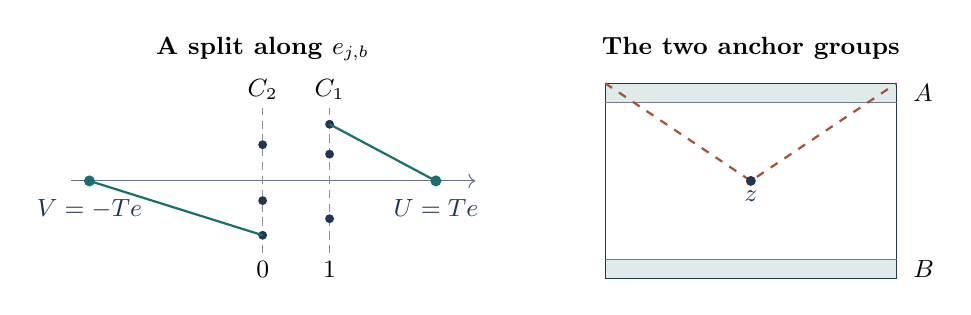
\begin{tikzpicture}[x=1cm,y=1cm,font=\small,
    wire/.style={draw=sea,thick},shadow/.style={draw=ink!55,densely dashed}]
  \node[font=\small\bfseries] at (0,1.68) {A split along \(e_{j,b}\)};
  \draw[draw=ink!70,->] (-2.44,0)--(2.7,0);
  \draw[shadow] (0,-.92)--(0,.92);
  \draw[shadow] (.85,-.92)--(.85,.92);
  \node at (0,1.16) {\(C_2\)};
  \node at (.85,1.16) {\(C_1\)};
  \foreach \y in {-.69,-.25,.46}{\fill[ink] (0,\y) circle (1.6pt);}
  \foreach \y in {-.48,.34,.72}{\fill[ink] (.85,\y) circle (1.6pt);}
  \draw[wire] (-2.2,0)--(0,-.69) (.85,.72)--(2.2,0);
  \fill[sea] (-2.2,0) circle (2pt) node[below=3pt,text=ink] {\(V=-Te\)};
  \fill[sea] (2.2,0) circle (2pt) node[below=3pt,text=ink] {\(U=Te\)};
  \node at (0,-1.12) {\(0\)};
  \node at (.85,-1.12) {\(1\)};
  \begin{scope}[xshift=6.2cm]
    \node[font=\small\bfseries] at (0,1.68) {The two anchor groups};
    \fill[sea!14] (-1.85,1) rectangle (1.85,1.24);
    \fill[sea!14] (-1.85,-1.24) rectangle (1.85,-1);
    \draw[draw=ink] (-1.85,-1.24) rectangle (1.85,1.24);
    \draw[draw=ink!65] (-1.85,1)--(1.85,1)
                       (-1.85,-1)--(1.85,-1);
    \draw[draw=rust,thick,dashed] (-1.85,1.24)--(0,0)--(1.85,1.24);
    \fill[ink] (0,0) circle (1.8pt) node[below] {\(z\)};
    \node[anchor=west] at (1.94,1.12) {\(A\)};
    \node[anchor=west] at (1.94,-1.12) {\(B\)};
  \end{scope}
\end{tikzpicture}
\caption{At left, the two classes project to zero and one on the chosen
code axis. The highlighted wires carry their votes to opposite
destinations. At right, a projection of the prism onto its interval
and height coordinates shows both anchor layers. Adding a central
site \(z\) to the upper anchor places the dashed triangle in the
projection of its hull. Distances and thicknesses are schematic.}
\label{fig:vote-layout}
\end{figure}

All \(v_i\) and all destinations lie in the cross-polytope
\(T B_1^m\), which has only \(2m\) vertices. For independent standard Gaussian coordinates \(g_j\), its mean width satisfies
\[
 \delta(TB_1^m)=\sqrt{2\pi}\,T\,\E\max_{j\le m}|g_j|
       \le \sqrt{2\pi}\,T\sqrt{2\ln(2m)} .
\]
Indeed, for \(u>0\) the expected
exponential of \(u\max_j|g_j|\) is at most \(2m e^{u^2/2}\).
Taking logarithms and minimizing the resulting upper bound on the
mean gives the inequality. Scale all positions by
\(\gamma=10^{-5}/(d\sqrt{\log(2m)})\). The resulting polytope
\(K=\gamma T B_1^m\) has \(\delta(K)\le10^{-3}\), and the wire gap
is at least \(0.9\gamma\).

\emph{Setting the anchor widths.}
Take the prism
\[
       P=P_0\times[-h,h],\qquad P_0=[-1,1]\times K,\qquad h=1.025
\]
in orthogonal coordinates. The central polytope consists of points
\((0,x,0)\) with \(x\in K\). Place the satellites at
\((0,\gamma v_i,0)\), the destinations at \((0,\pm\gamma Te,0)\),
and \(O\) at the origin. The upper anchor \(A\) contains all vertices
of \(P_0\) at height \(h\), and the lower anchor \(B\) contains their
reflections at \(-h\). Together these vertices span \(P\). We will
add sites only inside the prism, fixing the normalizing denominator
\[
       D=\delta(S)=\delta(P)=\delta(P_0)+2h,\qquad
       2\le\delta(P_0)=2+\delta(K)\le2.001 .
\]
In particular \(4.05\le D\le4.051\). Set \(\rho=\gamma/32\).
After normalization the wire gap is at least \(0.9\gamma/D>4\rho\),
proving~\eqref{eq:split-gap}, and the central polytope has width at
most \(10^{-3}/D\).

For each \(s=\rho,2\rho\), include in each anchor a second copy of
its vertices, a distance \(t_s\) toward the center. Its hull is
a product of \(P_0\) with an interval of length \(t_s\), giving width
\((\delta(P_0)+t_s)/D\). The choice
\[
       t_s=\tfrac12(1-s)D-\delta(P_0)
           =\tfrac12\bigl(2h-\delta(P_0)-sD\bigr)
\]
lies between \(0\) and \(0.03\) and gives the desired normalized
width \((1-s)/2\). Both choices use the same outer faces.

If \(z=(0,x,0)\) is central, the hull of \(A\cup\{z\}\) contains
the triangle joining \(z\) to \((-1,0,h)\) and \((1,0,h)\) in the
outer face. Its raw width is its semiperimeter,
\(1+\sqrt{1+h^2+\|x\|^2}>2.4\). Thus \(w(A\cup\{z\})>2.4/D>0.56\),
whereas \(w(A)\le1/2\). Reflection gives the same gain for \(B\).

For \(s=\rho\), append to each anchor one more layer a distance
\(\alpha D\) farther inward and to each satellite one more site at
height \(\alpha D\) above it. Each anchor hull grows by an interval
of length \(\alpha D\), and each satellite group becomes a segment of
that length. Hence each of the \(r\) widths increases by exactly
\(\alpha\). The anchor layers stay within \(0.04\) of their respective
outer faces, and different satellite groups have different projections
onto \(K\). The groups remain disjoint, and their union still spans
\(P\). Their surplus is therefore
\[
                  1-\bigl(1-\rho+r\alpha\bigr)=9\rho/10 .
\]
Each layer has \(4m\) vertices. Each original anchor has two layers,
and only a constant number of layers is needed altogether. Including
the satellites, their extra sites, the destinations and \(O\) gives
\(|S|=O(r+dq)\) and the stated bound on \(\ell\).
\end{proof}

\section{Eliminating anchor repetitions and large majorities}\label{sec:guard}

The recursion will look for a repeated letter among the satellites and
call a smaller test on the satellites that carry its head. Two cases
need separate treatment. A repeat can involve an anchor, and a letter
can occupy so many satellite sites that such a call would scarcely
reduce their number. We construct a gate, called the \emph{guard}, that
kills either kind of column whenever its entries do not all agree.

Fix either pair \(A,B\) of anchor groups in Lemma~\ref{lem:layout}, with
surplus \(s\in\{\rho,2\rho\}\). An anchor holds one \(b\)-bit letter,
replicated at every site of the group. Each satellite holds a \(b\)-bit
letter and an activity flag. Exactly \(n\ge2\) satellites are active.
\emph{Agreement} means that the two anchor letters and all \(n\)
active letters coincide.

\subsection{Choosing the two voting classes}

Order the at most \(dq\) coordinate--symbol classes of the satellite
code. Choose the first class \(C_1\) for which both \(C_1\) and its
complement \(C_2\) contain at least \(4p_0n\) active satellites, where
\(p_0=1/(128q)\). Lemma~\ref{lem:layout} ensures that a choice exists.
The index of this split and the two active counts are its \emph{split
data}. The data specify the voting classes, their destinations \(U,V\),
and the number of voters for each application of Lemma~\ref{lem:vote}.

\begin{lemma}[Computing the split]\label{lem:splitdata}
On the domain with \(n\) active satellites, a gate of price
\(G=O(dqH)\) appends the split data as basis controls at every site.
\end{lemma}
\begin{proof}
Sum over proposed vectors of active counts for all the code classes,
discarding vectors with no qualifying split. For each proposal
multiply the count tests of Equation~\eqref{eq:count-test}, one for
the activity flags in each class. This costs at most \(dq\log(r+1)\).
From the proposed vector and the public integer \(n\), each site
can write the same split data locally. There are at most
\((n+1)^{dq}\) proposals, so summing their gates adds at most
\(dq\log(n+1)\) to the price. Exactly one proposal passes on each
basis input, with coefficient one.
\end{proof}

\subsection{The guard}

\begin{lemma}[Guard]\label{lem:guard}
Suppose every site has the correct split data for the \(n\) active
satellites. For either anchor pair there is a gate of net cost at most
\[
       g_0=O\bigl(H+\log(2|S|)+\ell/\rho\bigr)
\]
uniformly in \(n,b\). It returns a fixed nonzero tensor on agreement.
On any other column it vanishes if either anchor letter occurs twice
or more among the two anchors and active satellites, or if a letter
occurs on more than \((1-p_0)n\) active satellites.
\end{lemma}

\begin{proof}
At \(b=0\) every column agrees, so use the unit gate. Assume \(b\ge1\)
and denote the anchor letters by \(a_A,a_B\). The guard combines three
tests on the original controls. A zero from any one of them kills the
whole column.

\emph{Equal anchors.}
Apply the promise broadcast of Lemma~\ref{lem:broadcast}(iii) from
\(A\cup B\) to all other sites. Its net cost is \(O(\log(2|S|))\)
because \(w(A\cup B)=1\). At every active satellite compare its letter
with the received label. Whenever \(a_A=a_B\), this comparison passes
exactly on agreement. Keep the broadcast registers. On agreement they
hold the common letter also at inactive sites, a fact we will use to
make the last test's output independent of that letter.

\emph{An anchor letter among the satellites.}
Suppose some active satellite holds \(a_A\). We will compare the two
anchor letters by projecting them onto the groups \(A\cup\{O\}\)
and \(B\), where \(O\) is the central site. Let \(\pi\) be any public
projection to \(u\) bits, put \(x=\pi(a_A)\), and let \(z_i\) be the
projection of satellite \(i\)'s letter. The anchors produce their own
projected labels locally. To produce \(x\) at \(O\), we select one
representative for each distinct \(z_i\) among active satellites and
weight those representatives by a polynomial in \(x\).

Fix an order on the satellites. Sum over \(i\), checking its activity.
Supply a partial diagonal of size \(2^u\) on \(O\) and all satellites,
and select its label \(z_i\) at \(i\). This costs at most \(10^{-3}u\)
by Lemma~\ref{lem:layout}. Each earlier active satellite can now
compare its projection with \(z_i\). Kill the branch if any matches.
Embed the projected alphabet in the working field and put
\[
        P_i(X)=
        \prod_{\substack{j\ \mathrm{active}\\z_j\ne z_i}}
                         \frac{X-z_j}{z_i-z_j}.
\]
For a surviving representative, \(P_i\) is one at its own label and
zero at every other active projected label. To apply the multiplier
\(P_i(x)\), choose \(r+1\) distinct field elements and interpolate in
\(X\). At each evaluation point, satellite \(j\) contributes its own
factor, since it holds both \(z_j\) and \(z_i\). A designated site in
\(A\) supplies the Lagrange coefficient at \(x\). The working field
is infinite and \(\deg P_i\le r\), so this calculation is exact in
every characteristic. Erase the temporary labels except for the copy
at \(O\). On the promise, \(x\) occurs, and exactly one representative
contributes, with coefficient one. This holds even if the projection
identifies several distinct input letters.

The sum over representatives and interpolation points adds \(O(H)\)
to the price. The projected-label gate therefore costs
\(10^{-3}u+O(H)\) and has unit auxiliary tensor. The two output
groups have union of width one. Their individual widths sum to at
least \(1-s+0.06\), since adjoining \(O\) increases the width of \(A\)
by at least \(0.06\). As \(s\le2\rho<0.002\), Lemma~\ref{lem:oracle}
applies with \(\lambda=10^{-3}\) and \(\sigma=0.05\). At net cost
\(O(H+\log(2|S|))\), it enforces \(a_A=a_B\) whenever an active
satellite holds \(a_A\). Repeat the construction with \(A,B\)
interchanged. If an anchor letter occurs twice, these tests and the
equal-anchor test leave only full agreement.

\emph{A large satellite majority.}
Sum over the split index and the active count in \(C_1\). Check these
against the stored split data before running the branch. The \(n\)
active votes are then divided between two specified classes with
known positive counts. Suppose \(y\) occurs at more than
\((1-p_0)n\) active satellites. There are fewer than \(p_0n\)
dissenting votes altogether and at least \(4p_0n\) voters in each
class. Thus \(y\) has more than three quarters of the active votes
in each class.

Apply Lemma~\ref{lem:vote} to send \(\pi(y)\) from \(C_1\) to \(U\)
and from \(C_2\) to \(V\). Together with the local projections of
the anchor letters, these operations give a projected-label gate for
\(a_A,a_B,y\) on the three groups \(A,B,\{U,V\}\). Its auxiliary
tensor \(J\) is the product of the two voter tensors and, on the
promise, is independent of \(u,\pi\). Let \(j\) be the sum of their
allowances. The gate costs at most \(j+\lambda u+O(H)\), where
Equation~\eqref{eq:split-gap} gives
\[
 \lambda=\max_{i\in C_1} w(\{x_i,U\})
           +\max_{i\in C_2} w(\{x_i,V\})
           \le w(\{U,V\})-4\rho .
\]
All three groups together have width one. Their individual widths sum
to at least \(1+\lambda+4\rho-s\). For the pair \(A,B\), the union
exceeds the sum by \(s\). For either anchor and \(\{U,V\}\), adjoining
\(U\) already increases the width by at least \(0.06\), while
\(w(\{U,V\})\le10^{-3}\). Thus Lemma~\ref{lem:oracle} applies with
\(\sigma=\rho\). On the majority promise this test vanishes unless
\(a_A=a_B=y\), in which case the equal-anchor test requires full
agreement.

On agreement every satellite has a retained broadcast copy of \(y\).
Use it to permute the local symbol slots in the two voter tensors as
in Lemma~\ref{lem:vote}, then erase the broadcast registers. For each
branch the permuted \(J\) is fixed, nonzero, and has price at least
\(j-O(H)\). Including it in the branch offset therefore recovers the
allowances to within \(O(H)\). The other offsets are already fixed.
Supply all unused branches' offsets in each branch before summing.
Exactly one split check passes, so the agreement output is independent
of the activity pattern as well as of \(y\). The at most \(dq(n+1)\)
branches cost \(O(H)\) to sum. The three oracle groups contain at most
\(|A|+|B|+2\) sites, so their contribution to the cost in
Lemma~\ref{lem:oracle} is \(O(H+\log(2|S|)+\ell/\rho)\).
\end{proof}

A violation that survives the guard has distinct anchor letters, each
occurring only once, and a repeated letter among the active satellites.
No satellite letter occupies more than \((1-p_0)n\) active sites.
Section~\ref{sec:masks} uses these facts to correct false ties. Shortening
the letters leaves the activity flags, and hence the existing split data,
in place. A recursive call that changes the active set pays \(G\) once
for its new split, then \(g_0\) for its guard.

\section{Shortening a column and correcting false ties}\label{sec:masks}

Splitting a letter into a head and a tail lets us run a shorter test.
We shift each tail by a mask depending only on its head. Two equal
letters have equal shifted tails for every choice of masks. Consequently,
on a violating column, the shorter test can survive only if all shifted
tails agree. We subtract exactly the mask choices that produce such a
false tie. The saving comes from a head containing two copies of the
same original letter. Figure~\ref{fig:example} in
Section~\ref{sec:design} illustrates the shorter test at that head.

Fix either pair of anchor groups \(A,B\) from Lemma~\ref{lem:layout}.
They have \(w(A\cup B)=1\) and \(w(A)+w(B)=1-s\), with
\(s\in\{\rho,2\rho\}\). A column consists of the two anchor letters,
each shared throughout its group, and the \(n\) active satellite
letters, where \(2\le n\le r-2\). Each satellite knows its activity
bit. Every site holds the split data of Lemma~\ref{lem:splitdata} for
these bits. Write \(f_s(b,n)\) for an achievable nonnegative upper
bound on the net cost of a gate for \(b\)-bit letters. The gate has one
fixed nonzero offset on agreement and vanishes on every violation. Its
cost bound holds for every column in this domain, and the offset is
independent of the active set.

\begin{lemma}[Mask recursion]\label{lem:mask-recursion}
A net cost of \(s b\) is achievable. Take \(g_0\) to be a sufficiently
large absolute constant times \(H+\log(2|S|)+\ell/\rho\), and let
\(G\) be the installation cost of Lemma~\ref{lem:splitdata}. For
\(1\le l\le b\) put \(b'=b-l\) and
\(\mathcal N_n=\{n'\in\mathbb Z:2\le n'\le(1-p_0)n\}\).
Given achievable bounds at length \(b'\), there is a gate at length
\(b\) with bound
\begin{equation}\label{eq:recursion}
\begin{aligned}
f_s(b,n) \le g_0+\max\Big\{&
  f_s(b',n),\\[-2pt]
& s b'+\max_{\substack{1\le j\le r\\ n'\in\mathcal N_n}}
 j\big(3l+g_0+G+f_{2\rho}(b',n')-2\rho b'\big)\Big\}.
\end{aligned}
\end{equation}
An empty maximum has value \(-\infty\).
\end{lemma}

\begin{proof}
For the first bound, test equality of the two anchors at cost \(s b\)
by Lemma~\ref{lem:broadcast}(i). The surviving anchors share one
letter on their union of width one. Broadcasting from this union
costs zero, and each active satellite can compare its own letter with
the broadcast copy locally. This gives the exact agreement predicate.
An equality test or broadcast on a zero-bit label uses the unit gate.

For the recursive bound, apply the guard of Lemma~\ref{lem:guard}.
A \emph{surviving violation} is a violating input on which the guard
is nonzero. On such an input each anchor letter occurs just once.
Some full satellite letter occurs at least twice, and every full
letter occurs on at most \((1-p_0)n\) active satellites. All gates
retain the original controls, so the two terms of a cancellation can
be checked on each basis input and tensored with the same guard output.

\smallskip\noindent\emph{Which masks need to be subtracted?}
Write \(\mathcal A=\{0,1\}^l\) for the heads and \(V=\mathbb F_2^{b'}\)
for the tails. Addition in \(V\) describes only the labels and works
over every coefficient field. Supply
\[
                   D=\bigotimes_{a\in\mathcal A}G_S(2^{b'}),
\]
one independent full diagonal of masks \(m_a\in V\) per head. Retain
the masks, compute \(v_i+m_{a_i}\) locally from each letter
\((a_i,v_i)\), and apply the \((b',n,s)\) gate to the shifted
tails. The active set and its split data are unchanged. On agreement
every mask tuple passes, so after erasing the temporary tails the
output is \(D\otimes Q\), where \(Q\) is the shorter gate's offset.
The main term costs at most \(f_s(b',n)\) relative to this output.

On a surviving violation a repeated full letter gives repeated shifted
tails. The child then returns either zero or \(Q\), with \(Q\) occurring
precisely when all shifted tails tie at some \(z\in V\). For fixed \(z\),
the mask required by an occurrence \((a,v_i)\) is \(m_a=v_i+z\).
The tensor of allowed masks in slot \(a\) is therefore
\begin{equation}\label{eq:mask-check}
 I_a(z)=
 \begin{cases}
 G_S(2^{b'}), & \text{if head \(a\) is absent},\\
 E_S(v+z),    & \text{if head \(a\) is occupied and all its tails equal \(v\)},\\
 0,           & \text{if head \(a\) has two different tails}.
 \end{cases}
\end{equation}
Only anchors and active satellites count as occurrences. For a surviving
violation the main output is
\(\big(\sum_{z\in V}\bigotimes_a I_a(z)\big)\otimes Q\).
Indeed, every mask tuple causing a tie determines a unique \(z\) and
has coefficient one in this sum.

A tie also requires the two anchor heads to be distinct and absent
among the active satellites. Another occurrence of either head would
have a different tail, since the corresponding anchor letter occurs
only once. In the correction, sum over the ordered pair of distinct
anchor heads and check their values and their absence at the active
satellites locally. On agreement no such branch passes. On a surviving
violation that can tie, exactly one passes.

\smallskip\noindent\emph{The cost of a repeat.}
Within a passing branch, supply \(z\) on a full diagonal at cost \(b'\).
For each anchor head, form its mask \(v_A+z\) or \(v_B+z\) throughout
the corresponding anchor and broadcast it by Lemma~\ref{lem:broadcast}(i).
Compared with supplying its full mask diagonal in \(D\), this saves
\(w(A)b'\) or \(w(B)b'\). Thus the two anchor masks leave \(s b'\) of
the cost of \(z\) to be paid.

To realize \(I_a(z)\) exactly for a non-anchor head \(a\), supply a
full mask diagonal and check \(m_a=v_i+z\) locally at each occurrence. Its cost is at most \(b'\).
We construct a second operation \(T_a(z)\) that will agree with the
exact one, up to a fixed offset, whenever head \(a\) contains a
repeated full letter of a surviving violation.

Flag the active satellites whose head is \(a\). For each
\(n'\in\mathcal N_n\), use the count predicate~\eqref{eq:count-test} to
select columns with exactly \(n'\) new flags. Install the corresponding
split data at cost \(G\) on the surviving support. Give the two inner
anchor groups independent dummy labels \(u,t\in V\) by supplying a
partial diagonal on each group. A newly flagged satellite receives
\(v_i+z\), and the other satellites can use any fixed local letter.
Apply the \((b',n',2\rho)\) gate and then broadcast from the union of
the inner anchors by Lemma~\ref{lem:broadcast}(iii). Keep the labels
in the mask slot at the sources and the broadcast copies in that slot
at every other site. The broadcast has its prescribed output when
\(u=t\), and its cost bound holds for every pair \(u,t\). Erase the
dummy inputs, new split data and temporary satellite letters.

Pad the count branches by the offsets of their unused child and
broadcast gates, as in Section~\ref{sec:prices}. Summing the branches
defines \(T_a(z)\) with common comparison offset \(Q_a\), the product
of these offsets over all allowed counts. Put
\(\widehat I_a(z)=I_a(z)\otimes Q_a\). If \(\mathcal N_n\) is empty,
take \(T_a=0\) and \(Q_a\) to be the unit. The offsets can be chosen
for every head independently of the guessed anchor heads.

To compare the two operations, suppose that head \(a\) contains a
repeated full letter in a surviving violation. Its count is at least
two. If its count exceeds \((1-p_0)n\), the guard ensures that at
least two tails in it differ. Then \(I_a(z)=0\), and \(T_a(z)=0\)
because no count branch passes. At an allowed count, the child
contains two equal satellite inputs for every pair of dummies. It
vanishes unless \emph{all} its inputs agree. Differing tails again
give zero on both sides. For common tail \(v\), exactly
\(u=t=v+z\) passes. That term gives the fixed child offset and
broadcasts the prescribed mask. The count and split selectors have
coefficient one. Thus, at every non-anchor head containing a repeated full letter
of a surviving violation,
\begin{equation}\label{eq:discount-agreement}
                    T_a(z)=\widehat I_a(z)\qquad(z\in V).
\end{equation}

Measure the cost of \(T_a\) against \(b'+h(Q_a)\), the price allowed
for the padded exact slot. The dummy diagonals have total price
\((1-2\rho)b'\). Selecting and summing the counts costs \(O(H)\).
The full-width broadcast has net cost \(O(\log(2|S|))\).
Including installation of the new split data and the child gate, the
excess cost is at most
\begin{equation}\label{eq:head-cost}
 G+O\big(H+\log(2|S|)\big)
   +\max_{n'\in\mathcal N_n}\big(f_{2\rho}(b',n')-2\rho b'\big).
\end{equation}
Padding charges each unused offset equally to the cost and the
comparison price.

\smallskip\noindent\emph{Cancellation across heads.}
For the guessed anchor heads \(a_A,a_B\), let
\(\mathcal H=\mathcal A\setminus\{a_A,a_B\}\). In the correction,
pad both anchor mask slots by their \(Q_a\)'s and supply \(Q\).
On the remaining slots use
\begin{equation}\label{eq:head-product}
 \bigotimes_{a\in\mathcal H}\widehat I_a(z)
 -
 \bigotimes_{a\in\mathcal H}\big(\widehat I_a(z)-T_a(z)\big).
\end{equation}
On every surviving violation passing the head checks, a repeated
full letter belongs to a non-anchor head. Equation~\eqref{eq:discount-agreement}
makes the second product zero, whatever the other \(T_a\)'s return.
Consequently the correction summed over \(z\) exactly reproduces the
padded main output on that violation. A surviving violation failing the head
checks could never tie. Agreement has equal anchor heads and so gives
no correction. Subtract the correction from the main term padded by
\(\bigotimes_a Q_a\). With the guard, the gate now vanishes on every
violation. Its fixed agreement offset is the tensor product of
\(D\), \(Q\), all the \(Q_a\)'s and the guard offset.

In the expansion of~\eqref{eq:head-product} the all-exact term cancels.
Each remaining summand uses \(T_a\) on some \(j\ge1\) distinct heads,
paying the excess~\eqref{eq:head-cost} at each of them. For a nonzero
summand, each of these heads has at least two active satellites.
Disjointness gives \(j\le\lfloor n/2\rfloor\), and there are at most
\(2^l-2\) non-anchor heads. In particular we may use \(j\le r\) in
the bound. There are at most \(2^{jl}\) subsets of size \(j\) and
\(2^{2l}\) ordered choices of anchor heads. Their logarithmic cost is
at most \((j+2)l\le3jl\). Add the residual \(s b'\) from \(z\).
Summing over \(j\), subtracting the correction and applying the guard
cost \(O(H)+O(H+\log(2|S|)+\ell/\rho)\). The main term needed no new
split. Absorbing these fixed charges in \(g_0\) gives~\eqref{eq:recursion}.
\end{proof}

\section{A gate of bounded cost for every alphabet}\label{sec:recurrence}

The alphabet enters the mask recursion only through the number \(b\)
of bits needed to name a letter. We will obtain three successive cost
bounds in \(b\). On the inner anchors, of surplus \(2\rho\), a linear
bound with slope \(\rho/4\) suffices. A call on these anchors replaces a
mask diagonal and saves \(2\rho\) per remaining bit before paying for the
call. This saving gives a logarithmic bound on the original anchors, of
surplus \(\rho\). Finally, the small increase in each group's width
given by Lemma~\ref{lem:layout} makes the cost bounded independently of
\(b\).

\subsection{Two estimates for the recursive test}

Use the overheads \(g_0,G\) of Lemma~\ref{lem:mask-recursion}. The
unchanged active set costs \(g_0\) at a recursive step. A call on a
smaller active set must also pay \(G\) to install its split data. For
\(n\) active satellites put
\[
 D(n)=\left\lfloor\frac{\log n}{-\log(1-p_0)}\right\rfloor,\qquad
 l_0=\lceil4g_0/\rho\rceil,\qquad
 A_j=10(l_0+G)(j+1).
\]
Every eligible smaller set has \(D(n')\le D(n)-1\), since
\(n'\le(1-p_0)n\). Put \(D_*=\lceil H\rceil+D(r)\) and \(A_*=A_{D_*}\).
In the binary layout \(p_0=1/256\), so \(D_*=O(H)\). The additional
\(\lceil H\rceil\) in this definition ensures
\(A_*\ge (g_0/\rho)H\).

\begin{lemma}[Linear and logarithmic costs]\label{lem:two-rates}
For every \(b\ge0\) and \(2\le n\le r-2\), the gates of
Section~\ref{sec:masks} on the groups of surplus \(2\rho\) and \(\rho\)
admit the respective net cost bounds
\begin{align}
 f_{2\rho}(b,n)&\le A_{D(n)}+\rho b/4, \label{eq:inner-rate}\\
 f_\rho(b,n)&\ll A_*+(g_0/\rho)\log(2+\rho b/A_*).
 \label{eq:root-rate}
\end{align}
\end{lemma}
\begin{proof}
For \eqref{eq:inner-rate}, induct on \(b\), simultaneously for all
\(n\), and set \(D=D(n)\). The exact comparison of
Lemma~\ref{lem:mask-recursion} costs \(2\rho b\), which proves the
claim when \(7\rho b/4\le A_D\). Above this threshold we have
\(l_0\le b\). Take \(l=l_0\), \(b'=b-l\) in \eqref{eq:recursion}.
In the main branch the linear bound decreases by
\(\rho l/4\ge g_0\), enough to pay the overhead.

If a correction has an eligible child, \(D\ge1\), and the cost
increment in \eqref{eq:recursion} for each head using such a child
is at most
\[
  3l+g_0+G+A_{D-1}-7\rho b'/4
  < (3+7\rho/4)l+g_0+G-(A_D-A_{D-1})<0 .
\]
Here \(A_D-A_{D-1}=10(l+G)\). At least one head must use the child.
The largest upper bound therefore occurs with one. Including the
outside costs \(g_0+2\rho b'\), the correction costs at most
\[
 A_{D-1}+3l+2g_0+G+\rho b'/4\ \le\ A_D+\rho b/4 .
\]
This proves the first estimate, including the case with no eligible child.

For \eqref{eq:root-rate}, use the exact comparison while
\(\rho b\le100A_*\). At greater lengths take
\(l=\lceil\rho b/50\rceil\) and \(b'=b-l\). By \eqref{eq:inner-rate}
the increment for each head using a child is at most
\[
  3l+g_0+G+A_*-7\rho b'/4\ \le\ -\rho b .
\]
Indeed \(l\le\rho b/50+1\), \(g_0+G\le A_*\), and
\(0<\rho<10^{-3}\). This pays even the full outside charge \(\rho b'\)
of the correction. Equation~\eqref{eq:recursion} thus gives
\(f_\rho(b,n)\le g_0+f_\rho(b',n)\), using nonnegative cost bounds.
Each such step leaves \(b'\le(1-\rho/50)b\) bits. It takes at most
\(O(\rho^{-1}\log(2+\rho b/A_*))\) steps to reach the exact comparison,
whose cost there is at most \(100A_*\).
\end{proof}

\subsection{Removing the dependence on the bit length}

Enlarge each of the \(r\) groups in the layout of surplus \(\rho\) by
the width increment \(\alpha=\rho/(10r)\) of Lemma~\ref{lem:layout}.
Every satellite participates in this final construction. We can still
call the gate on the original groups, with cost bound
\(f(t)=f_\rho(t,r-2)\) from \eqref{eq:root-rate}. Its activity flags
are all one, so its split data are fixed. The wider groups give the
exact checks a saving proportional to \(t\), which will dominate
\(f(t)\).

\begin{lemma}[Uniform cost in the alphabet]\label{lem:uniform-mask}
On the enlarged groups, for every \(b\ge0\) there is a gate of net
cost \(F(b)\ll A_*\) satisfying Lemma~\ref{lem:diagonal} on the full
domain of replicated \(b\)-bit letters. It returns a fixed nonzero
tensor on a constant column and zero on every column with a repeated
letter and at least two different letters.
\end{lemma}
\begin{proof}
At \(b=0\) the unit gate has \(F(0)=0\). For the step from \(t\)
to \(t+1\) bits, write each letter as \((a,v)\), where
\(a\in\{0,1\}\), \(v\in\mathbb F_2^t\). Supply two independent
full mask diagonals with labels \(m_0,m_1\in\mathbb F_2^t\).
Keep both mask slots and apply the shorter enlarged-group gate to the
letters \(v+m_a\). On a constant column its return is both full
diagonals times the shorter gate's offset \(Q\). Its net cost against
this offset is \(F(t)\).

On an inadmissible column a repeated original letter stays repeated
after masking. Thus a mask pair contributes only when every masked
tail equals one common value \(z\). Both heads must then occur.
Otherwise adding the same mask to every tail preserves the original
disagreement. We reproduce these surviving terms exactly, without the
guard of Section~\ref{sec:guard}, so the repeat may involve an anchor.

\paragraph{The two occupied heads.}
Sum over the two anchor head bits and check them locally. If they
are equal, also sum over the first satellite of the other head, checking
its head and checking the opposite bit at every earlier satellite.
When both heads occur exactly one branch passes, and when only one
occurs none passes. The logarithm of the number of branches is \(O(H)\).
In a passing branch sum over a public \(t\)-bit label \(z\). For each
\(a\in\{0,1\}\), the exact mask output \(I_a(z)\) is \(E_S(v+z)\)
if all letters with head \(a\) have a common tail \(v\), and is zero
otherwise. Since both heads are occupied, the tensor
\(\sum_z I_0(z)\otimes I_1(z)\) supplies exactly the mask pairs that
produce a common masked tail. Every such pair occurs once.

Let \(u_a\) be the sum of the widths of the \emph{original} anchors
with head \(a\), so \(u_0+u_1=1-\rho\). The exact output \(I_a(z)\)
can be produced at cost at most \((1-u_a-\alpha)t\).
With one anchor of head \(a\), broadcast its tail from the enlarged
anchor. With no anchor of this head, broadcast from its designated
enlarged satellite, of width \(\alpha\). In either case compare the
broadcast tail with every member of the head and add \(z\) locally
to form the mask. If both anchors have head \(a\), first compare their
tails at cost \((\rho-2\alpha)t\). On the surviving domain their
union, of width one, broadcasts the common tail at zero cost.
These operations use the domain version of Lemma~\ref{lem:broadcast}.

\paragraph{An alternative output at a repeated head.}
Construct \(T_a(z)\) on the original groups. Give each member of head
\(a\) its letter \(v+z\), and independently sum over a dummy \(t\)-bit
letter for each member of the other head. A dummy satellite is summed
at its single original site by the local vector \(\sum_v e_v\).
A dummy anchor requires a partial diagonal, so the dummy cost is
\((1-\rho-u_a)t\). Each satellite, real or dummy, takes part in the
call of cost \(f(t)\). Its original site can choose locally between
the real letter and the dummy sum. Thus the call uses the fixed split
data for all \(r-2\) satellites.

Apply the promise broadcast from the two original anchors, keep its
output in the mask slot, and erase the temporary registers. When the
anchors agree, every site receives their common letter.
Lemma~\ref{lem:broadcast}(iii) bounds the net cost on the whole
domain by \(O(\log(2|S|))\). The gate and broadcast offsets have a fixed
product \(P_a\), padded across public branches if necessary.
Thus \(T_a(z)\) has net cost at most
\[
       (1-\rho-u_a)t+f(t)+O(\log(2|S|)).
\]
Pad the exact output to \(\widehat I_a(z)=I_a(z)\otimes P_a\).

Suppose a pair of equal original letters has head \(a\). The input
of the original-group gate then already contains a repeat, whatever
the dummies are. It can survive only if all its inputs agree.
If two real tails in this head differ there is no surviving term.
If every real tail has value \(v\), the unique surviving assignment
sets every dummy to \(v+z\), and the broadcast acts on its promise.
In either case \(T_a(z)=\widehat I_a(z)\).

For each \(z\) use the correction
\[
 \widehat I_0(z)\otimes\widehat I_1(z)
 -
 \big(\widehat I_0(z)-T_0(z)\big)\otimes
 \big(\widehat I_1(z)-T_1(z)\big).
\]
At every inadmissible column with both heads present the second
product is zero, since one head contains a repeat. This conclusion
holds for every output of the other head's broadcast away from its
promise. Summing the first product over \(z\) therefore recovers
the surviving terms of the main branch. Append \(Q\) to the
correction and \(P_0\otimes P_1\) to the main branch, then subtract.
On inadmissible columns with a single head both branches already
vanish. On a constant column the correction vanishes and the return
is \(G_S(2^t)^{\otimes2}\otimes Q\otimes P_0\otimes P_1\).

\paragraph{Summing the costs.}
The product of the two exact outputs cancels in the expansion of the
correction. Every remaining summand uses one or two of the cheaper
outputs \(T_a\). Relative to the price \(t+h(P_a)\) of its slot in
the common offset, an exact head saves at least \((u_a+\alpha)t\).
A head using \(T_a\) contributes at most
\(f(t)-(u_a+\rho)t+O(\log(2|S|))\). Pay \(t\) for the shared \(z\).
Since \(u_0+u_1=1-\rho\), the resulting recurrence is
\begin{equation}\label{eq:outer-sum}
 F(t+1)\le
 \operatorname{lsum}\!\left(F(t),\;
 Cg_0+\max\{f(t)-\alpha t,\;2f(t)-\rho t\}\right),
\end{equation}
where \(\operatorname{lsum}(x,y)=\log_2(2^x+2^y)\) and \(C\) is
absolute. The first correction cost uses one \(T_a\), the second
uses both. All public choices and the sum of the three surviving
terms are included in \(Cg_0\).

Set \(x=\rho t/A_*\). Since \(A_*\ge(g_0/\rho)H\) and
\(\log r\le H\), the logarithmic term in \eqref{eq:root-rate} costs
\(O(A_*)\) up to \(x=r\). For all \(x\ge0\), use
\(\log(2+x)\le\log r+\log(2+x/r)\) and
\(\log(2+y)\le C_\delta+\delta y\). Choosing \(\delta>0\) small
enough gives
\[
                     f(t)\le C_1 A_*+\alpha t/8 .
\]
Both correction costs in \eqref{eq:outer-sum} are therefore at most
\(C_2 A_*-\alpha t/2\), including the overhead. Iterating after
exponentiation gives
\[
  2^{F(b)}
     \le 1+2^{C_2 A_*}\sum_{t=0}^{b-1}2^{-\alpha t/2}
     \le 1+O(2^{C_2 A_*}/\alpha).
\]
Finally \(\log(1/\alpha)=\log(10r/\rho)=O(A_*)\) by
Lemma~\ref{lem:layout}. This proves the bound uniformly in \(b\).
\end{proof}

\subsection{The bound for sets}

\begin{proof}[Proof of Theorem~\ref{thm:main}]
Let \(r\ge4\), and take a nonempty sunflower-free family of \(N\)
words of length \(k\). Embed the alphabet of each coordinate in a
binary cube, choosing the length independently at each coordinate.
Lemma~\ref{lem:uniform-mask} gives a gate of net cost \(O(A_*)\)
for each cube. The enlarged groups have surplus \(9\rho/10\).
Lemma~\ref{lem:diagonal} now gives
\[
                         (9\rho/10)\log_2 N\ll k A_* .
\]
In the binary layout \(d\ll H\), \(\ell\ll L\), \(\log |S|\ll H\),
and \(\rho^{-1}\ll H\sqrt L\) by Lemma~\ref{lem:layout}. The split
cost \(G=O(dqH)\) of Lemma~\ref{lem:splitdata} is \(O(H^2)\), and
the guard and summation overheads give
\[
 g_0/\rho\ll H/\rho+\ell/\rho^2\ll H^2 L^2,\qquad
 A_*\ll H(g_0/\rho+G)\ll H^3L^2 .
\]
Hence \(\log_2 N\ll kH^4L^{5/2}\). For \(r=3\) the fixed planar
construction in Section~\ref{sec:plane} gives \(\log_2 N=O(k)\).

For a \(k\)-uniform set family the coloring in Section~\ref{sec:words}
retains at least an \(e^{-k}\) fraction of its members as words.
Multiplication by \(e^k\) is absorbed by the absolute constant in
\(B_r\). For sets of size at most \(k\), pad each member to size \(k\)
with fresh elements belonging only to that member. Padding preserves
all intersections between distinct members, so the bound applies to
the original family as well.
\end{proof}

The diagonal comparison also applies when a word family contains
sunflowers, provided a tensor on the word indices can annihilate their
contributions. This costs only once for a whole tuple of words.

\begin{corollary}[A tensor vanishing on sunflowers]\label{cor:weighted}
Let \(r\ge3\) and let \(\mathcal W\) consist of \(N\ge1\) distinct words
of length \(k\). Suppose an order-\(r\) array over the working field,
indexed by \(\mathcal W^r\), has tensor rank \(R\), equals one on the
diagonal, and vanishes on every nondiagonal tuple admissible in
every coordinate. Then
\[
        \log_2 N\ll kH^4L^{5/2}+H\sqrt L\,\log_2 R .
\]
\end{corollary}
\begin{proof}
Multiply each joint word-index term in the diagonal comparison by
the specified array entry. For a simple tensor, one representative
of each group multiplies by its factor locally. Summing over a rank
decomposition costs at most \(\log_2 R\). The coordinate gates kill
every tuple with an inadmissible column. The array kills the remaining
nondiagonal tuples, and its diagonal entries preserve the common
offset. Thus \((9\rho/10)\log_2 N\ll k A_*+\log_2 R\) for \(r\ge4\).
For \(r=3\) apply the same weighting to the planar comparison of
Proposition~\ref{prop:comparison}, with the three groups of
Section~\ref{sec:plane}. Their positive surplus and the total
cost per coordinate are absolute constants, giving
\(\log_2 N\ll k+\log_2 R\).
\end{proof}

The optimal base \(b_r=\sup_{k\ge1}M_r(k)^{1/k}\) is also the limiting
growth rate as \(k\to\infty\) by the product construction of
Abbott~\cite[Theorem~1]{Abbott66}. Take sunflower-free uniform
families of respective set sizes \(k,l\) on disjoint ground sets, and
form all unions of a member of each. If \(r\) of the unions formed a
sunflower, their projections to either ground set would have constant
pairwise intersection. If two projections there were equal, that
common intersection would be the entire projected set. By uniformity
every projection containing it would equal it. If no two were equal,
the projections would themselves be a sunflower. Thus both projections
would be constant, contradicting distinctness of the unions.
Consequently \(M_r(k+l)\ge M_r(k)M_r(l)\), and Fekete's
lemma applied to \(\log M_r(k)\) gives
\[
                         b_r=\lim_{k\to\infty}M_r(k)^{1/k}.
\]
The block transversals in the introduction give \(b_r\ge r-1\).
Whether \(b_r=O(r)\) remains open.


\bibliographystyle{plainnat}
\bookmarksetup{startatroot}
\bibliography{references}
\end{document}
